\documentclass[twoside]{book}

% Packages required by doxygen
\usepackage{fixltx2e}
\usepackage{calc}
\usepackage{doxygen}
\usepackage[export]{adjustbox} % also loads graphicx
\usepackage{graphicx}
\usepackage[utf8]{inputenc}
\usepackage{makeidx}
\usepackage{multicol}
\usepackage{multirow}
\PassOptionsToPackage{warn}{textcomp}
\usepackage{textcomp}
\usepackage[nointegrals]{wasysym}
\usepackage[table]{xcolor}

% Font selection
\usepackage[T1]{fontenc}
\usepackage[scaled=.90]{helvet}
\usepackage{courier}
\usepackage{amssymb}
\usepackage{sectsty}
\renewcommand{\familydefault}{\sfdefault}
\allsectionsfont{%
  \fontseries{bc}\selectfont%
  \color{darkgray}%
}
\renewcommand{\DoxyLabelFont}{%
  \fontseries{bc}\selectfont%
  \color{darkgray}%
}
\newcommand{\+}{\discretionary{\mbox{\scriptsize$\hookleftarrow$}}{}{}}

% Page & text layout
\usepackage{geometry}
\geometry{%
  a4paper,%
  top=2.5cm,%
  bottom=2.5cm,%
  left=2.5cm,%
  right=2.5cm%
}
\tolerance=750
\hfuzz=15pt
\hbadness=750
\setlength{\emergencystretch}{15pt}
\setlength{\parindent}{0cm}
\setlength{\parskip}{0.2cm}
\makeatletter
\renewcommand{\paragraph}{%
  \@startsection{paragraph}{4}{0ex}{-1.0ex}{1.0ex}{%
    \normalfont\normalsize\bfseries\SS@parafont%
  }%
}
\renewcommand{\subparagraph}{%
  \@startsection{subparagraph}{5}{0ex}{-1.0ex}{1.0ex}{%
    \normalfont\normalsize\bfseries\SS@subparafont%
  }%
}
\makeatother

% Headers & footers
\usepackage{fancyhdr}
\pagestyle{fancyplain}
\fancyhead[LE]{\fancyplain{}{\bfseries\thepage}}
\fancyhead[CE]{\fancyplain{}{}}
\fancyhead[RE]{\fancyplain{}{\bfseries\leftmark}}
\fancyhead[LO]{\fancyplain{}{\bfseries\rightmark}}
\fancyhead[CO]{\fancyplain{}{}}
\fancyhead[RO]{\fancyplain{}{\bfseries\thepage}}
\fancyfoot[LE]{\fancyplain{}{}}
\fancyfoot[CE]{\fancyplain{}{}}
\fancyfoot[RE]{\fancyplain{}{\bfseries\scriptsize Generated on Thu Oct 15 2015 22\+:28\+:18 for toy\+Engine3\+D by Doxygen }}
\fancyfoot[LO]{\fancyplain{}{\bfseries\scriptsize Generated on Thu Oct 15 2015 22\+:28\+:18 for toy\+Engine3\+D by Doxygen }}
\fancyfoot[CO]{\fancyplain{}{}}
\fancyfoot[RO]{\fancyplain{}{}}
\renewcommand{\footrulewidth}{0.4pt}
\renewcommand{\chaptermark}[1]{%
  \markboth{#1}{}%
}
\renewcommand{\sectionmark}[1]{%
  \markright{\thesection\ #1}%
}

% Indices & bibliography
\usepackage{natbib}
\usepackage[titles]{tocloft}
\setcounter{tocdepth}{3}
\setcounter{secnumdepth}{5}
\makeindex

% Hyperlinks (required, but should be loaded last)
\usepackage{ifpdf}
\ifpdf
  \usepackage[pdftex,pagebackref=true]{hyperref}
\else
  \usepackage[ps2pdf,pagebackref=true]{hyperref}
\fi
\hypersetup{%
  colorlinks=true,%
  linkcolor=blue,%
  citecolor=blue,%
  unicode%
}

% Custom commands
\newcommand{\clearemptydoublepage}{%
  \newpage{\pagestyle{empty}\cleardoublepage}%
}


%===== C O N T E N T S =====

\begin{document}

% Titlepage & ToC
\hypersetup{pageanchor=false,
             bookmarks=true,
             bookmarksnumbered=true,
             pdfencoding=unicode
            }
\pagenumbering{roman}
\begin{titlepage}
\vspace*{7cm}
\begin{center}%
{\Large toy\+Engine3\+D }\\
\vspace*{1cm}
{\large Generated by Doxygen 1.8.10}\\
\vspace*{0.5cm}
{\small Thu Oct 15 2015 22:28:18}\\
\end{center}
\end{titlepage}
\clearemptydoublepage
\tableofcontents
\clearemptydoublepage
\pagenumbering{arabic}
\hypersetup{pageanchor=true}

%--- Begin generated contents ---
\chapter{Hierarchical Index}
\section{Class Hierarchy}
This inheritance list is sorted roughly, but not completely, alphabetically\+:\begin{DoxyCompactList}
\item \contentsline{section}{Actor}{\pageref{class_actor}}{}
\begin{DoxyCompactList}
\item \contentsline{section}{Enemy}{\pageref{class_enemy}}{}
\end{DoxyCompactList}
\item \contentsline{section}{Attribute}{\pageref{class_attribute}}{}
\item \contentsline{section}{Camera}{\pageref{class_camera}}{}
\begin{DoxyCompactList}
\item \contentsline{section}{Perspective\+Camera}{\pageref{class_perspective_camera}}{}
\begin{DoxyCompactList}
\item \contentsline{section}{Player\+Camera}{\pageref{class_player_camera}}{}
\end{DoxyCompactList}
\end{DoxyCompactList}
\item \contentsline{section}{Font\+:\+:Char\+Info}{\pageref{struct_font_1_1_char_info}}{}
\item \contentsline{section}{Collider}{\pageref{class_collider}}{}
\begin{DoxyCompactList}
\item \contentsline{section}{Sphere}{\pageref{class_sphere}}{}
\begin{DoxyCompactList}
\item \contentsline{section}{Enemy}{\pageref{class_enemy}}{}
\end{DoxyCompactList}
\item \contentsline{section}{Terrain}{\pageref{class_terrain}}{}
\end{DoxyCompactList}
\item \contentsline{section}{Curve$<$ T $>$}{\pageref{class_curve}}{}
\item \contentsline{section}{Curve$<$ G\+Lfloat $>$}{\pageref{class_curve}}{}
\item \contentsline{section}{Curve$<$ glm\+:\+:vec2 $>$}{\pageref{class_curve}}{}
\item \contentsline{section}{Curve$<$ glm\+:\+:vec3 $>$}{\pageref{class_curve}}{}
\item \contentsline{section}{Curve$<$ glm\+:\+:vec4 $>$}{\pageref{class_curve}}{}
\item \contentsline{section}{Font}{\pageref{class_font}}{}
\item \contentsline{section}{Framebuffer}{\pageref{class_framebuffer}}{}
\item \contentsline{section}{Height\+Map}{\pageref{class_height_map}}{}
\item \contentsline{section}{Mesh\+Data}{\pageref{class_mesh_data}}{}
\item \contentsline{section}{Particle}{\pageref{class_particle}}{}
\item \contentsline{section}{Point\+Light}{\pageref{class_point_light}}{}
\item \contentsline{section}{Renderable}{\pageref{class_renderable}}{}
\begin{DoxyCompactList}
\item \contentsline{section}{Billboard}{\pageref{class_billboard}}{}
\item \contentsline{section}{Lighting}{\pageref{class_lighting}}{}
\item \contentsline{section}{Mesh}{\pageref{class_mesh}}{}
\begin{DoxyCompactList}
\item \contentsline{section}{Enemy}{\pageref{class_enemy}}{}
\item \contentsline{section}{Terrain}{\pageref{class_terrain}}{}
\end{DoxyCompactList}
\item \contentsline{section}{Particle\+System}{\pageref{class_particle_system}}{}
\begin{DoxyCompactList}
\item \contentsline{section}{Bullet\+Spawner}{\pageref{class_bullet_spawner}}{}
\item \contentsline{section}{Light\+Well}{\pageref{class_light_well}}{}
\item \contentsline{section}{Smooth\+Tail}{\pageref{class_smooth_tail}}{}
\end{DoxyCompactList}
\item \contentsline{section}{Post\+Effect}{\pageref{class_post_effect}}{}
\begin{DoxyCompactList}
\item \contentsline{section}{Blend}{\pageref{class_blend}}{}
\item \contentsline{section}{Bloom}{\pageref{class_bloom}}{}
\end{DoxyCompactList}
\item \contentsline{section}{Text}{\pageref{class_text}}{}
\end{DoxyCompactList}
\item \contentsline{section}{Shader}{\pageref{class_shader}}{}
\item \contentsline{section}{Texture}{\pageref{class_texture}}{}
\item \contentsline{section}{World}{\pageref{class_world}}{}
\end{DoxyCompactList}

\chapter{Class Index}
\section{Class List}
Here are the classes, structs, unions and interfaces with brief descriptions\+:\begin{DoxyCompactList}
\item\contentsline{section}{\hyperlink{class_actor}{Actor} }{\pageref{class_actor}}{}
\item\contentsline{section}{\hyperlink{class_attribute}{Attribute} }{\pageref{class_attribute}}{}
\item\contentsline{section}{\hyperlink{class_billboard}{Billboard} }{\pageref{class_billboard}}{}
\item\contentsline{section}{\hyperlink{class_blend}{Blend} }{\pageref{class_blend}}{}
\item\contentsline{section}{\hyperlink{class_bloom}{Bloom} }{\pageref{class_bloom}}{}
\item\contentsline{section}{\hyperlink{class_bullet_spawner}{Bullet\+Spawner} }{\pageref{class_bullet_spawner}}{}
\item\contentsline{section}{\hyperlink{class_camera}{Camera} }{\pageref{class_camera}}{}
\item\contentsline{section}{\hyperlink{struct_font_1_1_char_info}{Font\+::\+Char\+Info} }{\pageref{struct_font_1_1_char_info}}{}
\item\contentsline{section}{\hyperlink{class_collider}{Collider} }{\pageref{class_collider}}{}
\item\contentsline{section}{\hyperlink{class_curve}{Curve$<$ T $>$} }{\pageref{class_curve}}{}
\item\contentsline{section}{\hyperlink{class_enemy}{Enemy} }{\pageref{class_enemy}}{}
\item\contentsline{section}{\hyperlink{class_font}{Font} }{\pageref{class_font}}{}
\item\contentsline{section}{\hyperlink{class_framebuffer}{Framebuffer} }{\pageref{class_framebuffer}}{}
\item\contentsline{section}{\hyperlink{class_height_map}{Height\+Map} }{\pageref{class_height_map}}{}
\item\contentsline{section}{\hyperlink{class_lighting}{Lighting} }{\pageref{class_lighting}}{}
\item\contentsline{section}{\hyperlink{class_light_well}{Light\+Well} }{\pageref{class_light_well}}{}
\item\contentsline{section}{\hyperlink{class_mesh}{Mesh} }{\pageref{class_mesh}}{}
\item\contentsline{section}{\hyperlink{class_mesh_data}{Mesh\+Data} }{\pageref{class_mesh_data}}{}
\item\contentsline{section}{\hyperlink{class_particle}{Particle} }{\pageref{class_particle}}{}
\item\contentsline{section}{\hyperlink{class_particle_system}{Particle\+System} }{\pageref{class_particle_system}}{}
\item\contentsline{section}{\hyperlink{class_perspective_camera}{Perspective\+Camera} }{\pageref{class_perspective_camera}}{}
\item\contentsline{section}{\hyperlink{class_player_camera}{Player\+Camera} }{\pageref{class_player_camera}}{}
\item\contentsline{section}{\hyperlink{class_point_light}{Point\+Light} }{\pageref{class_point_light}}{}
\item\contentsline{section}{\hyperlink{class_post_effect}{Post\+Effect} }{\pageref{class_post_effect}}{}
\item\contentsline{section}{\hyperlink{class_renderable}{Renderable} }{\pageref{class_renderable}}{}
\item\contentsline{section}{\hyperlink{class_shader}{Shader} }{\pageref{class_shader}}{}
\item\contentsline{section}{\hyperlink{class_smooth_tail}{Smooth\+Tail} }{\pageref{class_smooth_tail}}{}
\item\contentsline{section}{\hyperlink{class_sphere}{Sphere} }{\pageref{class_sphere}}{}
\item\contentsline{section}{\hyperlink{class_terrain}{Terrain} }{\pageref{class_terrain}}{}
\item\contentsline{section}{\hyperlink{class_text}{Text} }{\pageref{class_text}}{}
\item\contentsline{section}{\hyperlink{class_texture}{Texture} }{\pageref{class_texture}}{}
\item\contentsline{section}{\hyperlink{class_world}{World} }{\pageref{class_world}}{}
\end{DoxyCompactList}

\chapter{Class Documentation}
\hypertarget{class_actor}{}\section{Actor Class Reference}
\label{class_actor}\index{Actor@{Actor}}


Inheritance diagram for Actor\+:\nopagebreak
\begin{figure}[H]
\begin{center}
\leavevmode
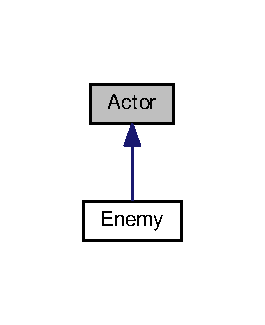
\includegraphics[width=127pt]{class_actor__inherit__graph}
\end{center}
\end{figure}


Collaboration diagram for Actor\+:\nopagebreak
\begin{figure}[H]
\begin{center}
\leavevmode
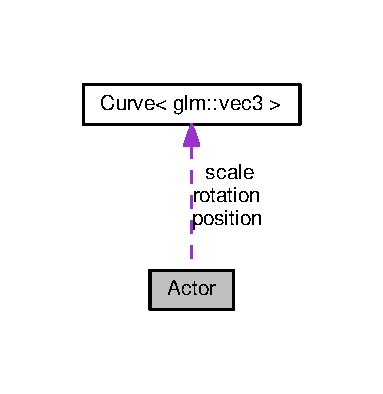
\includegraphics[width=184pt]{class_actor__coll__graph}
\end{center}
\end{figure}
\subsection*{Public Member Functions}
\begin{DoxyCompactItemize}
\item 
\hypertarget{class_actor_aca81671d1a816725523bf45e03167858}{}virtual void {\bfseries step} (float dt)\label{class_actor_aca81671d1a816725523bf45e03167858}

\item 
\hypertarget{class_actor_a77d4385e6144f842dd40b213e27d8aa1}{}glm\+::mat4 {\bfseries get\+Model} () const \label{class_actor_a77d4385e6144f842dd40b213e27d8aa1}

\end{DoxyCompactItemize}
\subsection*{Public Attributes}
\begin{DoxyCompactItemize}
\item 
\hypertarget{class_actor_a5acb451a91aa2cdc6abfb877d60a65e1}{}\hyperlink{class_curve}{Curve}$<$ glm\+::vec3 $>$ {\bfseries position}\label{class_actor_a5acb451a91aa2cdc6abfb877d60a65e1}

\item 
\hypertarget{class_actor_ac6d54863e68a37c67e83ab876ea82bc6}{}\hyperlink{class_curve}{Curve}$<$ glm\+::vec3 $>$ {\bfseries scale}\label{class_actor_ac6d54863e68a37c67e83ab876ea82bc6}

\item 
\hypertarget{class_actor_ac388bcd18a687f53ab9926d9379b782c}{}\hyperlink{class_curve}{Curve}$<$ glm\+::vec3 $>$ {\bfseries rotation}\label{class_actor_ac388bcd18a687f53ab9926d9379b782c}

\end{DoxyCompactItemize}


The documentation for this class was generated from the following file\+:\begin{DoxyCompactItemize}
\item 
src/actor.\+h\end{DoxyCompactItemize}

\hypertarget{class_attribute}{}\section{Attribute Class Reference}
\label{class_attribute}\index{Attribute@{Attribute}}
\subsection*{Public Types}
\begin{DoxyCompactItemize}
\item 
\hypertarget{class_attribute_ab652b3f3bd344279f6f58b9fc8b0736d}{}enum {\bfseries Dimension} \{ {\bfseries scalar} = 1, 
{\bfseries vec2}, 
{\bfseries vec3}, 
{\bfseries vec4}
 \}\label{class_attribute_ab652b3f3bd344279f6f58b9fc8b0736d}

\end{DoxyCompactItemize}
\subsection*{Public Member Functions}
\begin{DoxyCompactItemize}
\item 
\hypertarget{class_attribute_a49656a9d8e78068ffab7fb9335243b40}{}{\bfseries Attribute} (G\+Lenum t, Dimension dim, G\+Lsizei s=0, const G\+Lvoid $\ast$o=0)\label{class_attribute_a49656a9d8e78068ffab7fb9335243b40}

\item 
\hypertarget{class_attribute_ab065aaf1fe2127c087a62f30167bdd03}{}{\bfseries Attribute} (G\+Luint buffer, G\+Lenum t, Dimension dim, G\+Lsizei s=0, const G\+Lvoid $\ast$o=0)\label{class_attribute_ab065aaf1fe2127c087a62f30167bdd03}

\item 
\hypertarget{class_attribute_ad3c383ce9cd15736d536d1cbc1cec088}{}void {\bfseries delete\+Data} ()\label{class_attribute_ad3c383ce9cd15736d536d1cbc1cec088}

\item 
\hypertarget{class_attribute_a6d4901774d60df8795ab7b5fbefd4ecc}{}void {\bfseries load\+Data} (void $\ast$data, size\+\_\+t n, G\+Lenum hint)\label{class_attribute_a6d4901774d60df8795ab7b5fbefd4ecc}

\end{DoxyCompactItemize}
\subsection*{Public Attributes}
\begin{DoxyCompactItemize}
\item 
\hypertarget{class_attribute_a5eff3a5f5d606957c65579b952dacbbc}{}G\+Luint {\bfseries vbo}\label{class_attribute_a5eff3a5f5d606957c65579b952dacbbc}

\item 
\hypertarget{class_attribute_ad053c6716a9ad5686bf16dd0d96c3a38}{}G\+Lenum {\bfseries type}\label{class_attribute_ad053c6716a9ad5686bf16dd0d96c3a38}

\item 
\hypertarget{class_attribute_a1a2ccd748b39f5533a04d89e53de59f8}{}Dimension {\bfseries dim}\label{class_attribute_a1a2ccd748b39f5533a04d89e53de59f8}

\item 
\hypertarget{class_attribute_af80cc5c521bd8c158c0a8b56d83f11df}{}G\+Lsizei {\bfseries stride}\label{class_attribute_af80cc5c521bd8c158c0a8b56d83f11df}

\item 
\hypertarget{class_attribute_afbde769206a46942e1ab5f3181279668}{}const G\+Lvoid $\ast$ {\bfseries offset}\label{class_attribute_afbde769206a46942e1ab5f3181279668}

\item 
\hypertarget{class_attribute_a888e509f2b818bdd28368dfc198e53e9}{}G\+Luint {\bfseries divisor}\label{class_attribute_a888e509f2b818bdd28368dfc198e53e9}

\end{DoxyCompactItemize}


The documentation for this class was generated from the following files\+:\begin{DoxyCompactItemize}
\item 
src/renderable.\+h\item 
src/renderable.\+cpp\end{DoxyCompactItemize}

\hypertarget{class_billboard}{}\section{Billboard Class Reference}
\label{class_billboard}\index{Billboard@{Billboard}}


Inheritance diagram for Billboard\+:\nopagebreak
\begin{figure}[H]
\begin{center}
\leavevmode
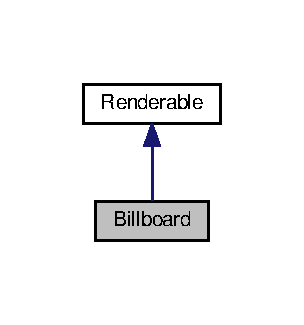
\includegraphics[width=146pt]{class_billboard__inherit__graph}
\end{center}
\end{figure}


Collaboration diagram for Billboard\+:\nopagebreak
\begin{figure}[H]
\begin{center}
\leavevmode
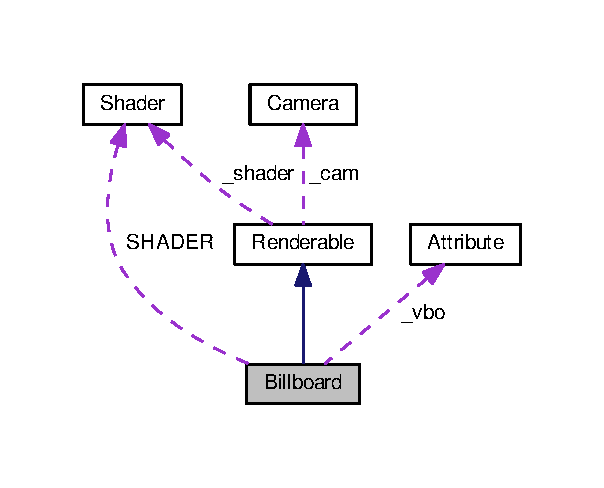
\includegraphics[width=290pt]{class_billboard__coll__graph}
\end{center}
\end{figure}
\subsection*{Public Member Functions}
\begin{DoxyCompactItemize}
\item 
\hypertarget{class_billboard_a41fcebb826ad9e284c633342c673d2cf}{}{\bfseries Billboard} (\hyperlink{class_camera}{Camera} $\ast$cam, G\+Luint texture)\label{class_billboard_a41fcebb826ad9e284c633342c673d2cf}

\item 
\hypertarget{class_billboard_aacd8d0899c6621377217554d7ac0610a}{}virtual void {\bfseries render} ()\label{class_billboard_aacd8d0899c6621377217554d7ac0610a}

\item 
\hypertarget{class_billboard_a2f3e5f1622b813c19cc81393522480a0}{}void {\bfseries set\+Position} (glm\+::vec3 pos)\label{class_billboard_a2f3e5f1622b813c19cc81393522480a0}

\item 
\hypertarget{class_billboard_a8f7bb38b293b16d94126ea5f5860afc7}{}glm\+::vec3 {\bfseries get\+Position} () const \label{class_billboard_a8f7bb38b293b16d94126ea5f5860afc7}

\item 
\hypertarget{class_billboard_a5803ecb146549666442a8d6612efd240}{}void {\bfseries set\+Size} (glm\+::vec2 size)\label{class_billboard_a5803ecb146549666442a8d6612efd240}

\item 
\hypertarget{class_billboard_aad09edf0a72fba9282d3608e9054641d}{}glm\+::vec2 {\bfseries get\+Size} () const \label{class_billboard_aad09edf0a72fba9282d3608e9054641d}

\end{DoxyCompactItemize}
\subsection*{Static Public Attributes}
\begin{DoxyCompactItemize}
\item 
\hypertarget{class_billboard_a4b6c53530979e84c9033c45ffdcaeb70}{}static \hyperlink{class_shader}{Shader} $\ast$ {\bfseries S\+H\+A\+D\+E\+R} = 0\label{class_billboard_a4b6c53530979e84c9033c45ffdcaeb70}

\end{DoxyCompactItemize}
\subsection*{Protected Attributes}
\begin{DoxyCompactItemize}
\item 
\hypertarget{class_billboard_aca662cbb29249fff9ce4ef70f3d4631c}{}G\+Luint {\bfseries \+\_\+texture}\label{class_billboard_aca662cbb29249fff9ce4ef70f3d4631c}

\item 
\hypertarget{class_billboard_aac80d99f04519704cf9a3dfa04283868}{}\hyperlink{class_attribute}{Attribute} {\bfseries \+\_\+vbo}\label{class_billboard_aac80d99f04519704cf9a3dfa04283868}

\item 
\hypertarget{class_billboard_a37a76361d3ff00534dce23e47cbc0051}{}glm\+::vec3 {\bfseries \+\_\+pos}\label{class_billboard_a37a76361d3ff00534dce23e47cbc0051}

\item 
\hypertarget{class_billboard_a665281e24fc18d9843b080a482d51cd0}{}glm\+::vec2 {\bfseries \+\_\+scale}\label{class_billboard_a665281e24fc18d9843b080a482d51cd0}

\end{DoxyCompactItemize}


The documentation for this class was generated from the following files\+:\begin{DoxyCompactItemize}
\item 
src/billboard.\+h\item 
src/billboard.\+cpp\end{DoxyCompactItemize}

\hypertarget{class_blend}{}\section{Blend Class Reference}
\label{class_blend}\index{Blend@{Blend}}


Inheritance diagram for Blend\+:\nopagebreak
\begin{figure}[H]
\begin{center}
\leavevmode
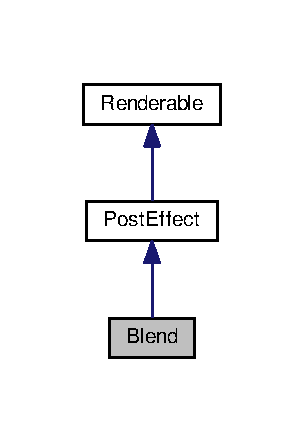
\includegraphics[width=146pt]{class_blend__inherit__graph}
\end{center}
\end{figure}


Collaboration diagram for Blend\+:\nopagebreak
\begin{figure}[H]
\begin{center}
\leavevmode
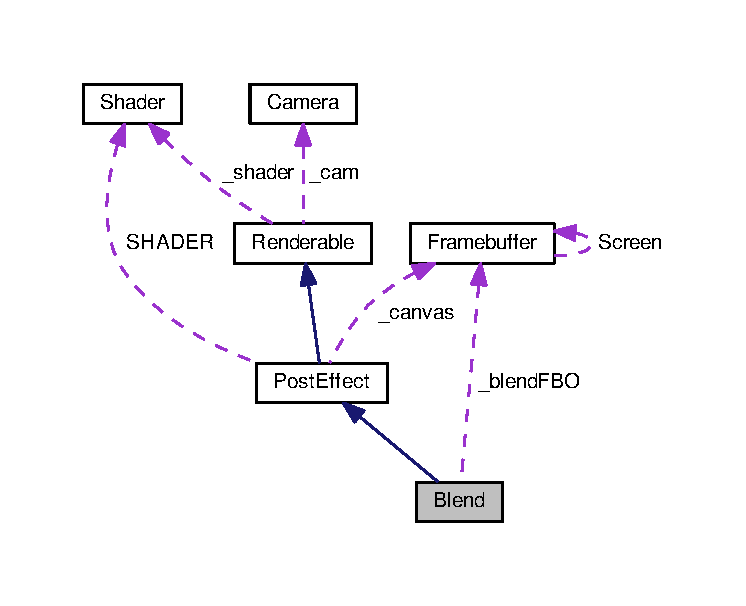
\includegraphics[width=350pt]{class_blend__coll__graph}
\end{center}
\end{figure}
\subsection*{Public Member Functions}
\begin{DoxyCompactItemize}
\item 
\hypertarget{class_blend_a808e2f2d6fd021ca43d22985d78d9465}{}{\bfseries Blend} (\hyperlink{class_framebuffer}{Framebuffer} $\ast$a, \hyperlink{class_framebuffer}{Framebuffer} $\ast$b)\label{class_blend_a808e2f2d6fd021ca43d22985d78d9465}

\item 
\hypertarget{class_blend_a5399ccf82cbcb03559bd9176f5959a84}{}virtual void {\bfseries render} ()\label{class_blend_a5399ccf82cbcb03559bd9176f5959a84}

\end{DoxyCompactItemize}
\subsection*{Protected Attributes}
\begin{DoxyCompactItemize}
\item 
\hypertarget{class_blend_ad557975355c427baaf87be7b91d6d7d8}{}\hyperlink{class_framebuffer}{Framebuffer} $\ast$ {\bfseries \+\_\+blend\+F\+B\+O}\label{class_blend_ad557975355c427baaf87be7b91d6d7d8}

\end{DoxyCompactItemize}
\subsection*{Additional Inherited Members}


The documentation for this class was generated from the following files\+:\begin{DoxyCompactItemize}
\item 
src/posteffect.\+h\item 
src/posteffect.\+cpp\end{DoxyCompactItemize}

\hypertarget{class_bloom}{}\section{Bloom Class Reference}
\label{class_bloom}\index{Bloom@{Bloom}}


Inheritance diagram for Bloom\+:\nopagebreak
\begin{figure}[H]
\begin{center}
\leavevmode
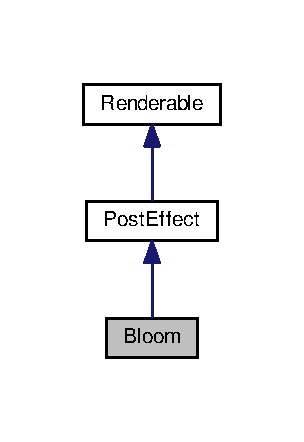
\includegraphics[width=146pt]{class_bloom__inherit__graph}
\end{center}
\end{figure}


Collaboration diagram for Bloom\+:\nopagebreak
\begin{figure}[H]
\begin{center}
\leavevmode
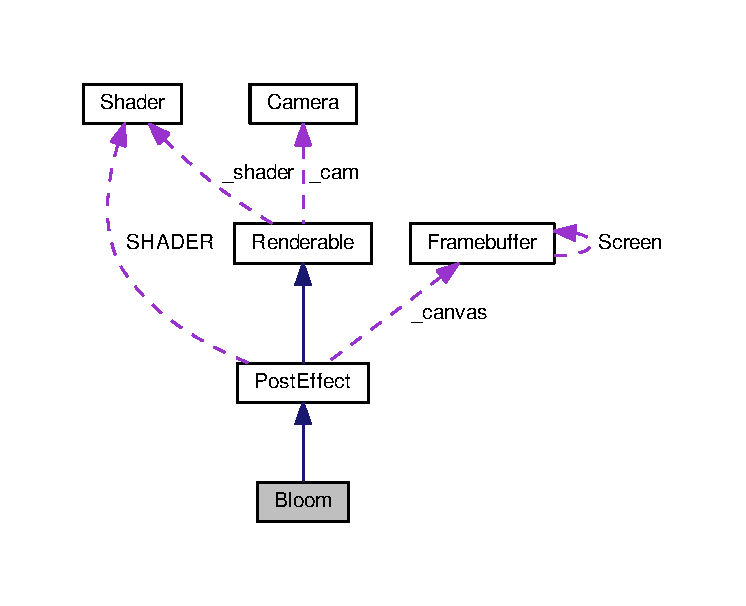
\includegraphics[width=350pt]{class_bloom__coll__graph}
\end{center}
\end{figure}
\subsection*{Public Member Functions}
\begin{DoxyCompactItemize}
\item 
\hypertarget{class_bloom_abfd2a3c58a5a62b8aa49fb953e5081e6}{}{\bfseries Bloom} (\hyperlink{class_framebuffer}{Framebuffer} $\ast$in, \hyperlink{class_framebuffer}{Framebuffer} $\ast$out)\label{class_bloom_abfd2a3c58a5a62b8aa49fb953e5081e6}

\item 
\hypertarget{class_bloom_a7754f494e4a503d4483215912efe6687}{}virtual void {\bfseries render} ()\label{class_bloom_a7754f494e4a503d4483215912efe6687}

\end{DoxyCompactItemize}
\subsection*{Additional Inherited Members}


The documentation for this class was generated from the following files\+:\begin{DoxyCompactItemize}
\item 
src/posteffect.\+h\item 
src/posteffect.\+cpp\end{DoxyCompactItemize}

\hypertarget{class_bullet_spawner}{}\section{Bullet\+Spawner Class Reference}
\label{class_bullet_spawner}\index{Bullet\+Spawner@{Bullet\+Spawner}}


Inheritance diagram for Bullet\+Spawner\+:\nopagebreak
\begin{figure}[H]
\begin{center}
\leavevmode
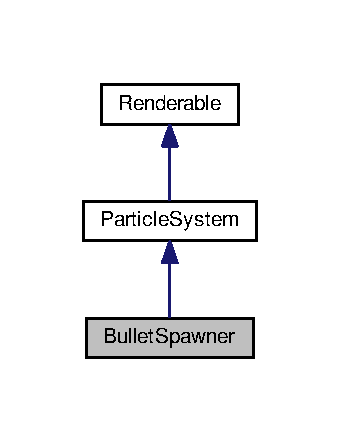
\includegraphics[width=163pt]{class_bullet_spawner__inherit__graph}
\end{center}
\end{figure}


Collaboration diagram for Bullet\+Spawner\+:\nopagebreak
\begin{figure}[H]
\begin{center}
\leavevmode
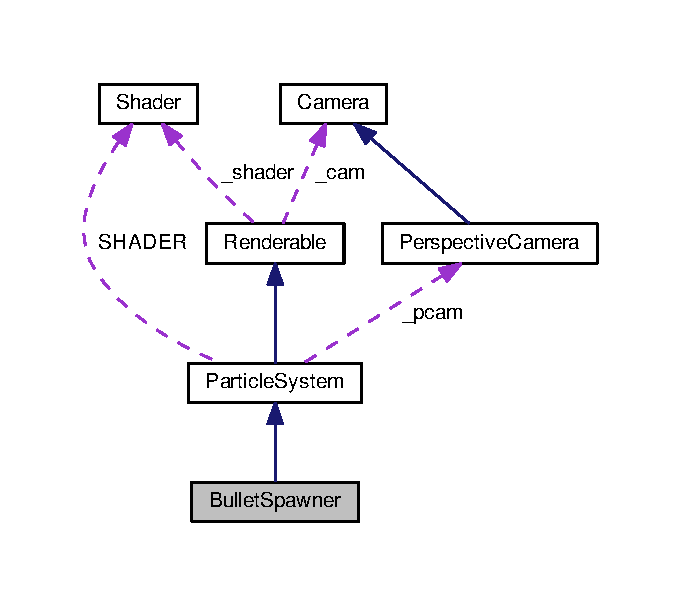
\includegraphics[width=327pt]{class_bullet_spawner__coll__graph}
\end{center}
\end{figure}
\subsection*{Public Member Functions}
\begin{DoxyCompactItemize}
\item 
\hypertarget{class_bullet_spawner_ae70bcc7f68643cc7c16fa82a864ad372}{}{\bfseries Bullet\+Spawner} (\hyperlink{class_perspective_camera}{Perspective\+Camera} $\ast$cam, std\+::vector$<$ \hyperlink{class_enemy}{Enemy} $\ast$ $>$ $\ast$enemies)\label{class_bullet_spawner_ae70bcc7f68643cc7c16fa82a864ad372}

\item 
\hypertarget{class_bullet_spawner_a5474e1659e4ca43f59620d31d53ed3d9}{}virtual void {\bfseries step} (double dt)\label{class_bullet_spawner_a5474e1659e4ca43f59620d31d53ed3d9}

\item 
\hypertarget{class_bullet_spawner_a2ef82c18cb619b1a23073f87453804f5}{}virtual void {\bfseries shoot} ()\label{class_bullet_spawner_a2ef82c18cb619b1a23073f87453804f5}

\end{DoxyCompactItemize}
\subsection*{Additional Inherited Members}


The documentation for this class was generated from the following files\+:\begin{DoxyCompactItemize}
\item 
src/particle.\+h\item 
src/particle.\+cpp\end{DoxyCompactItemize}

\hypertarget{class_camera}{}\section{Camera Class Reference}
\label{class_camera}\index{Camera@{Camera}}


Inheritance diagram for Camera\+:\nopagebreak
\begin{figure}[H]
\begin{center}
\leavevmode
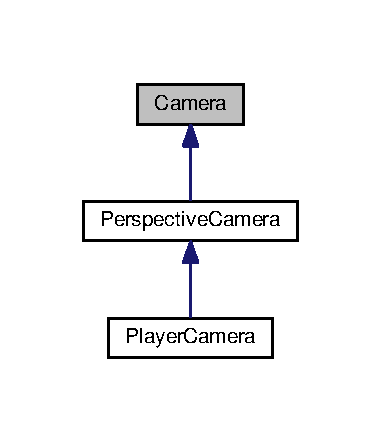
\includegraphics[width=183pt]{class_camera__inherit__graph}
\end{center}
\end{figure}
\subsection*{Public Member Functions}
\begin{DoxyCompactItemize}
\item 
\hypertarget{class_camera_ab4a79b59eed20caf458908239df811ba}{}virtual void {\bfseries set\+Uniforms} (\hyperlink{class_shader}{Shader} $\ast$shader) const \label{class_camera_ab4a79b59eed20caf458908239df811ba}

\end{DoxyCompactItemize}


The documentation for this class was generated from the following file\+:\begin{DoxyCompactItemize}
\item 
src/camera.\+h\end{DoxyCompactItemize}

\hypertarget{struct_font_1_1_char_info}{}\section{Font\+:\+:Char\+Info Struct Reference}
\label{struct_font_1_1_char_info}\index{Font\+::\+Char\+Info@{Font\+::\+Char\+Info}}
\subsection*{Public Attributes}
\begin{DoxyCompactItemize}
\item 
\hypertarget{struct_font_1_1_char_info_a2470f2ec8620001d4d32fe993a6904d5}{}float {\bfseries ax}\label{struct_font_1_1_char_info_a2470f2ec8620001d4d32fe993a6904d5}

\item 
\hypertarget{struct_font_1_1_char_info_abfbc6fc9aaec8abb8aff9c107c59dcca}{}float {\bfseries ay}\label{struct_font_1_1_char_info_abfbc6fc9aaec8abb8aff9c107c59dcca}

\item 
\hypertarget{struct_font_1_1_char_info_a0881be09b1f0079b63d051e668554411}{}float {\bfseries bw}\label{struct_font_1_1_char_info_a0881be09b1f0079b63d051e668554411}

\item 
\hypertarget{struct_font_1_1_char_info_ae9423ddaa245ecbd95472bff8513a581}{}float {\bfseries bh}\label{struct_font_1_1_char_info_ae9423ddaa245ecbd95472bff8513a581}

\item 
\hypertarget{struct_font_1_1_char_info_a533ae5ae1a3fcd8251eeb595825de0f0}{}float {\bfseries bl}\label{struct_font_1_1_char_info_a533ae5ae1a3fcd8251eeb595825de0f0}

\item 
\hypertarget{struct_font_1_1_char_info_a5520f6fc19d21a52bfd4575cc44f26e6}{}float {\bfseries bt}\label{struct_font_1_1_char_info_a5520f6fc19d21a52bfd4575cc44f26e6}

\item 
\hypertarget{struct_font_1_1_char_info_a86552e140407025d9b915ec5676e3cd9}{}float {\bfseries tx}\label{struct_font_1_1_char_info_a86552e140407025d9b915ec5676e3cd9}

\end{DoxyCompactItemize}


The documentation for this struct was generated from the following file\+:\begin{DoxyCompactItemize}
\item 
src/text.\+h\end{DoxyCompactItemize}

\hypertarget{class_collider}{}\section{Collider Class Reference}
\label{class_collider}\index{Collider@{Collider}}


Inheritance diagram for Collider\+:\nopagebreak
\begin{figure}[H]
\begin{center}
\leavevmode
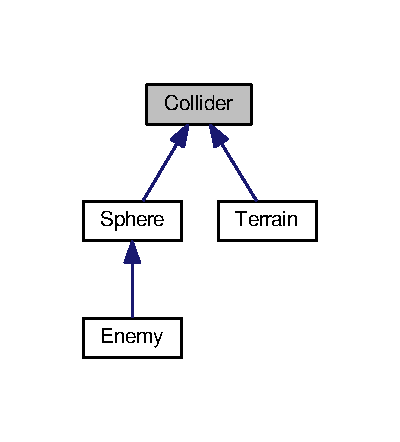
\includegraphics[width=192pt]{class_collider__inherit__graph}
\end{center}
\end{figure}
\subsection*{Public Member Functions}
\begin{DoxyCompactItemize}
\item 
\hypertarget{class_collider_ae852216c6d07c0221167a48d0d2f7020}{}virtual bool {\bfseries contains} (glm\+::vec3 point) const  =0\label{class_collider_ae852216c6d07c0221167a48d0d2f7020}

\item 
\hypertarget{class_collider_ad911610da1f4f9c28f66c4b3bedcce84}{}virtual glm\+::vec3 {\bfseries correct} (glm\+::vec3 point) const  =0\label{class_collider_ad911610da1f4f9c28f66c4b3bedcce84}

\end{DoxyCompactItemize}


The documentation for this class was generated from the following file\+:\begin{DoxyCompactItemize}
\item 
src/collider.\+h\end{DoxyCompactItemize}

\hypertarget{class_curve}{}\section{Curve$<$ T $>$ Class Template Reference}
\label{class_curve}\index{Curve$<$ T $>$@{Curve$<$ T $>$}}


Collaboration diagram for Curve$<$ T $>$\+:\nopagebreak
\begin{figure}[H]
\begin{center}
\leavevmode
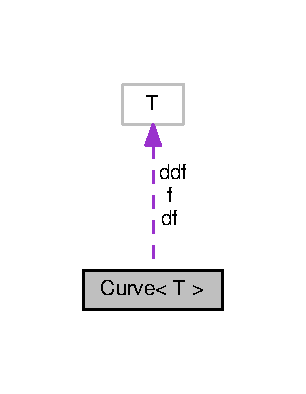
\includegraphics[width=147pt]{class_curve__coll__graph}
\end{center}
\end{figure}
\subsection*{Public Member Functions}
\begin{DoxyCompactItemize}
\item 
\hypertarget{class_curve_a3d0a8e023c4f32e0a81cd649b68bbbef}{}{\bfseries Curve} (T x0)\label{class_curve_a3d0a8e023c4f32e0a81cd649b68bbbef}

\item 
\hypertarget{class_curve_ae14fb9529abb405244b78219fce1d8c5}{}{\bfseries Curve} (T x0, T v0)\label{class_curve_ae14fb9529abb405244b78219fce1d8c5}

\item 
\hypertarget{class_curve_a8f65cc108b133951735ec1dcb67aae8b}{}{\bfseries Curve} (T x0, T v0, T a0)\label{class_curve_a8f65cc108b133951735ec1dcb67aae8b}

\item 
\hypertarget{class_curve_a93867fb84d32342fec79460c64339df4}{}void {\bfseries step} (float dt)\label{class_curve_a93867fb84d32342fec79460c64339df4}

\end{DoxyCompactItemize}
\subsection*{Public Attributes}
\begin{DoxyCompactItemize}
\item 
\hypertarget{class_curve_a02a72792f2bbfea110fbe01aa867886d}{}T {\bfseries f}\label{class_curve_a02a72792f2bbfea110fbe01aa867886d}

\item 
\hypertarget{class_curve_a6a8808bc765a4cb3e8dc3e55c9d85acc}{}T {\bfseries df}\label{class_curve_a6a8808bc765a4cb3e8dc3e55c9d85acc}

\item 
\hypertarget{class_curve_a339f0053ae5bd5b9bf8ae8cc2e0a558f}{}T {\bfseries ddf}\label{class_curve_a339f0053ae5bd5b9bf8ae8cc2e0a558f}

\end{DoxyCompactItemize}


The documentation for this class was generated from the following file\+:\begin{DoxyCompactItemize}
\item 
src/actor.\+h\end{DoxyCompactItemize}

\hypertarget{class_enemy}{}\section{Enemy Class Reference}
\label{class_enemy}\index{Enemy@{Enemy}}


Inheritance diagram for Enemy\+:\nopagebreak
\begin{figure}[H]
\begin{center}
\leavevmode
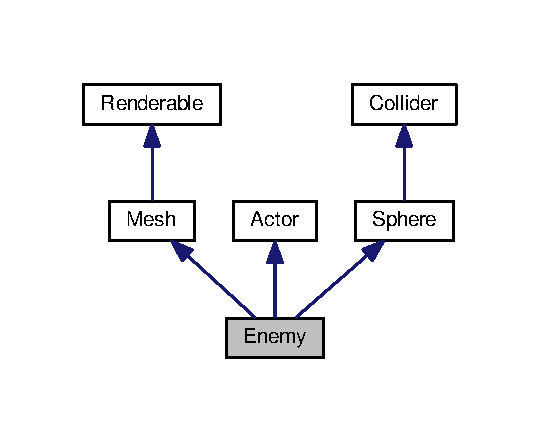
\includegraphics[width=259pt]{class_enemy__inherit__graph}
\end{center}
\end{figure}


Collaboration diagram for Enemy\+:\nopagebreak
\begin{figure}[H]
\begin{center}
\leavevmode
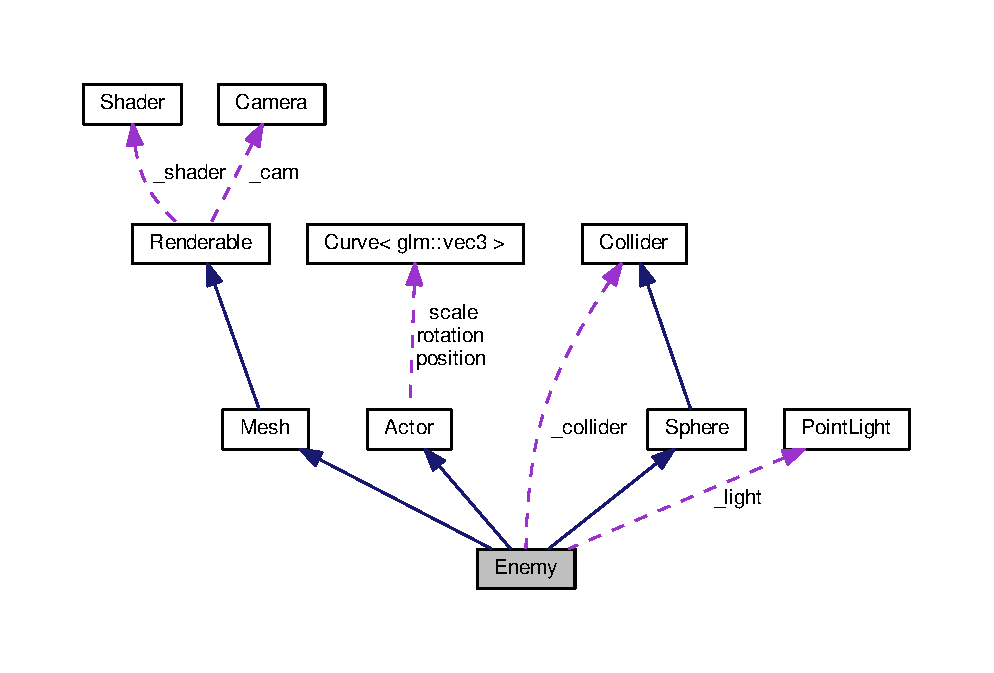
\includegraphics[width=350pt]{class_enemy__coll__graph}
\end{center}
\end{figure}
\subsection*{Public Member Functions}
\begin{DoxyCompactItemize}
\item 
\hypertarget{class_enemy_a510bb7f4bb1a38fefaef246c458e672a}{}{\bfseries Enemy} (\hyperlink{class_camera}{Camera} $\ast$cam, \hyperlink{class_mesh_data}{Mesh\+Data} $\ast$data, \hyperlink{class_collider}{Collider} $\ast$collider)\label{class_enemy_a510bb7f4bb1a38fefaef246c458e672a}

\item 
\hypertarget{class_enemy_ae741a4a1ba7097e42b6764923e82b8fc}{}virtual void {\bfseries step} (double dt)\label{class_enemy_ae741a4a1ba7097e42b6764923e82b8fc}

\item 
\hypertarget{class_enemy_a62875c8aba22d278c89caa87af6c7b69}{}virtual void {\bfseries render} ()\label{class_enemy_a62875c8aba22d278c89caa87af6c7b69}

\item 
\hypertarget{class_enemy_a116b78399fc93edf91ae2b20cb278a26}{}virtual void {\bfseries on\+Hit} ()\label{class_enemy_a116b78399fc93edf91ae2b20cb278a26}

\item 
\hypertarget{class_enemy_a2faed0e6daf8ca132f40c33e7b192a07}{}\hyperlink{class_point_light}{Point\+Light} \& {\bfseries point\+Light} ()\label{class_enemy_a2faed0e6daf8ca132f40c33e7b192a07}

\item 
\hypertarget{class_enemy_a0f2ab608b481d1f19f65e83f98eda591}{}bool {\bfseries is\+Alive} () const \label{class_enemy_a0f2ab608b481d1f19f65e83f98eda591}

\item 
\hypertarget{class_enemy_a01f4404cf0c0c38bb287241541c2cef1}{}void {\bfseries set\+Color} (glm\+::vec4 color)\label{class_enemy_a01f4404cf0c0c38bb287241541c2cef1}

\end{DoxyCompactItemize}
\subsection*{Protected Attributes}
\begin{DoxyCompactItemize}
\item 
\hypertarget{class_enemy_ab90b6580f551c2d344dcdd9848d3da0a}{}\hyperlink{class_collider}{Collider} $\ast$ {\bfseries \+\_\+collider}\label{class_enemy_ab90b6580f551c2d344dcdd9848d3da0a}

\item 
\hypertarget{class_enemy_a7bb871e6546c740a456613873f472e69}{}\hyperlink{class_point_light}{Point\+Light} {\bfseries \+\_\+light}\label{class_enemy_a7bb871e6546c740a456613873f472e69}

\item 
\hypertarget{class_enemy_acf28445e8f8aabedcc8cd248ca1b9588}{}bool {\bfseries \+\_\+alive}\label{class_enemy_acf28445e8f8aabedcc8cd248ca1b9588}

\end{DoxyCompactItemize}
\subsection*{Additional Inherited Members}


The documentation for this class was generated from the following files\+:\begin{DoxyCompactItemize}
\item 
src/body.\+h\item 
src/enemy.\+cpp\end{DoxyCompactItemize}

\hypertarget{class_font}{}\section{Font Class Reference}
\label{class_font}\index{Font@{Font}}


{\ttfamily \#include $<$text.\+h$>$}

\subsection*{Classes}
\begin{DoxyCompactItemize}
\item 
struct \hyperlink{struct_font_1_1_char_info}{Char\+Info}
\end{DoxyCompactItemize}
\subsection*{Public Member Functions}
\begin{DoxyCompactItemize}
\item 
\hypertarget{class_font_a0fc255ee986a505e9fa67baead2b5ad8}{}{\bfseries Font} (std\+::string name, int font\+Size)\label{class_font_a0fc255ee986a505e9fa67baead2b5ad8}

\item 
\hypertarget{class_font_ad2fa45002c535ee444a00bcaa28d7ab0}{}\hyperlink{struct_font_1_1_char_info}{Char\+Info} $\ast$ {\bfseries get\+Char\+Info} ()\label{class_font_ad2fa45002c535ee444a00bcaa28d7ab0}

\item 
\hypertarget{class_font_a0c776ec8dffad0cbfa512e55e7a69e76}{}G\+Luint {\bfseries get\+Atlas} () const \label{class_font_a0c776ec8dffad0cbfa512e55e7a69e76}

\item 
\hypertarget{class_font_a2a8f74ccaee05c104f26bc52163650fd}{}unsigned int {\bfseries get\+Atlas\+Height} () const \label{class_font_a2a8f74ccaee05c104f26bc52163650fd}

\item 
\hypertarget{class_font_acb8ec4718fca077a312a84410e84a38e}{}unsigned int {\bfseries get\+Atlas\+Width} () const \label{class_font_acb8ec4718fca077a312a84410e84a38e}

\item 
\hypertarget{class_font_a9933e8b7c09d73246f2b572b70ceb2bf}{}int {\bfseries get\+Size} () const \label{class_font_a9933e8b7c09d73246f2b572b70ceb2bf}

\end{DoxyCompactItemize}
\subsection*{Static Public Attributes}
\begin{DoxyCompactItemize}
\item 
\hypertarget{class_font_ae975f79e48736a286097d01c19f6fe6e}{}static F\+T\+\_\+\+Library {\bfseries ft} = 0\label{class_font_ae975f79e48736a286097d01c19f6fe6e}

\end{DoxyCompactItemize}


\subsection{Detailed Description}
\hyperlink{class_font}{Font} atlas stored on G\+P\+U 

The documentation for this class was generated from the following files\+:\begin{DoxyCompactItemize}
\item 
src/text.\+h\item 
src/text.\+cpp\end{DoxyCompactItemize}

\hypertarget{class_framebuffer}{}\section{Framebuffer Class Reference}
\label{class_framebuffer}\index{Framebuffer@{Framebuffer}}


Collaboration diagram for Framebuffer\+:\nopagebreak
\begin{figure}[H]
\begin{center}
\leavevmode
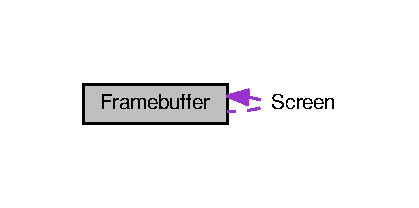
\includegraphics[width=201pt]{class_framebuffer__coll__graph}
\end{center}
\end{figure}
\subsection*{Public Member Functions}
\begin{DoxyCompactItemize}
\item 
\hyperlink{class_framebuffer_a4f10f2020d414add1ea0e6553908c86b}{Framebuffer} ()
\item 
\hyperlink{class_framebuffer_a46ec55ab64b360550afb2de19043852a}{Framebuffer} (G\+Luint fbo)
\item 
\hyperlink{class_framebuffer_aaed0ae64dc7a0b2762ce74d89913365a}{Framebuffer} (int w, int h)
\item 
\hyperlink{class_framebuffer_a037bf3e17455354d5d907ceea00313dd}{$\sim$\+Framebuffer} ()
\item 
void \hyperlink{class_framebuffer_a167694f148f4de766971234389f04b8a}{add\+Attachment} ()
\item 
void \hyperlink{class_framebuffer_a1cc8b67cd13927bfb88b52fe5886d580}{enable\+Depth\+Buffer} (G\+Lenum internal\+Format=G\+L\+\_\+\+D\+E\+P\+T\+H\+\_\+\+C\+O\+M\+P\+O\+N\+E\+N\+T16)
\item 
void \hyperlink{class_framebuffer_a4106324f9cffad333255ce5dab0d4c73}{bind\+Draw} () const 
\item 
void \hyperlink{class_framebuffer_a9f14f58040d7d242f28dad5aff1a5564}{bind\+Read} () const 
\item 
void \hyperlink{class_framebuffer_a9479ea40d39418a623f64d91b151163f}{resize} (int w, int h)
\item 
void \hyperlink{class_framebuffer_a2182f6f6c725b0efa128a6b5775241e8}{copy\+Color} (const \hyperlink{class_framebuffer}{Framebuffer} \&fb)
\item 
void \hyperlink{class_framebuffer_a3fdff897f598d2c659e251de3c8325da}{copy\+Depth} (const \hyperlink{class_framebuffer}{Framebuffer} \&fb)
\item 
void \hyperlink{class_framebuffer_a54aeea0a6f75c104fd974b0743cac55c}{clear\+Color} ()
\item 
void \hyperlink{class_framebuffer_a01944581e97067094ae7902c43da45ee}{clear\+Depth} ()
\item 
void \hyperlink{class_framebuffer_a29f3edfceab261b122f09a8a1b067b41}{clear} ()
\item 
G\+Luint \hyperlink{class_framebuffer_af19335525cae0fb92f20aa46f18d426c}{get\+F\+B\+O} () const 
\item 
\hypertarget{class_framebuffer_ab7fee6a15f7fc7fa9b8585d4c4c08f03}{}{\bfseries operator G\+Luint} ()\label{class_framebuffer_ab7fee6a15f7fc7fa9b8585d4c4c08f03}

\item 
std\+::vector$<$ \hyperlink{class_texture}{Texture} $\ast$ $>$ \& \hyperlink{class_framebuffer_aab2ffec3fc4c6d5efe71e2a8bea64f8b}{get\+Attachments} ()
\item 
int \hyperlink{class_framebuffer_a7b32671cc35241f0e8a75fe0565003d8}{get\+Width} () const 
\item 
int \hyperlink{class_framebuffer_ab1e7b6a5fb21ab0462536f823c97f7d1}{get\+Height} () const 
\end{DoxyCompactItemize}
\subsection*{Static Public Member Functions}
\begin{DoxyCompactItemize}
\item 
static \hyperlink{class_framebuffer}{Framebuffer} $\ast$ \hyperlink{class_framebuffer_add4c1f7b2a3eb1eb007c297b0ac0d88d}{gen\+Geometry\+Buffer} ()
\item 
static \hyperlink{class_framebuffer}{Framebuffer} $\ast$ \hyperlink{class_framebuffer_a6df15a90817f9f0b364d8a9c2050f481}{gen\+Screen\+Buffer} ()
\item 
static const \hyperlink{class_framebuffer}{Framebuffer} $\ast$ \hyperlink{class_framebuffer_ae6fe9b975e5a186087fcb53bcfbf7a9d}{get\+Active\+Draw} ()
\item 
static const \hyperlink{class_framebuffer}{Framebuffer} $\ast$ \hyperlink{class_framebuffer_a0871301296352207df787148de752a21}{get\+Active\+Read} ()
\end{DoxyCompactItemize}
\subsection*{Static Public Attributes}
\begin{DoxyCompactItemize}
\item 
\hypertarget{class_framebuffer_a0a8040e6caa0d5c207ccae24a99f89ce}{}static \hyperlink{class_framebuffer}{Framebuffer} \hyperlink{class_framebuffer_a0a8040e6caa0d5c207ccae24a99f89ce}{Screen} = \hyperlink{class_framebuffer}{Framebuffer}( 0 )\label{class_framebuffer_a0a8040e6caa0d5c207ccae24a99f89ce}

\begin{DoxyCompactList}\small\item\em The Screen \hyperlink{class_framebuffer}{Framebuffer}, has I\+D zero. \end{DoxyCompactList}\end{DoxyCompactItemize}
\subsection*{Protected Attributes}
\begin{DoxyCompactItemize}
\item 
\hypertarget{class_framebuffer_af27bf1f68f7da2b7b3c48190356245bc}{}int {\bfseries \+\_\+width}\label{class_framebuffer_af27bf1f68f7da2b7b3c48190356245bc}

\item 
\hypertarget{class_framebuffer_a63e2b3d16786239f6f2342733fc3b722}{}int {\bfseries \+\_\+height}\label{class_framebuffer_a63e2b3d16786239f6f2342733fc3b722}

\item 
\hypertarget{class_framebuffer_a542d8261ea8a78ac2777e7bfdedaaaab}{}G\+Luint \hyperlink{class_framebuffer_a542d8261ea8a78ac2777e7bfdedaaaab}{\+\_\+fbo}\label{class_framebuffer_a542d8261ea8a78ac2777e7bfdedaaaab}

\begin{DoxyCompactList}\small\item\em open\+G\+L I\+D \end{DoxyCompactList}\item 
\hypertarget{class_framebuffer_adfd7fb74d3dd0fac749000c5c888c6a6}{}G\+Luint \hyperlink{class_framebuffer_adfd7fb74d3dd0fac749000c5c888c6a6}{\+\_\+depth\+R\+B\+O}\label{class_framebuffer_adfd7fb74d3dd0fac749000c5c888c6a6}

\begin{DoxyCompactList}\small\item\em depth Renderbuffer open\+G\+L I\+D \end{DoxyCompactList}\item 
\hypertarget{class_framebuffer_ae2d9ec57440ab3201da60ff8f4f5f09a}{}std\+::vector$<$ \hyperlink{class_texture}{Texture} $\ast$ $>$ \hyperlink{class_framebuffer_ae2d9ec57440ab3201da60ff8f4f5f09a}{\+\_\+attachments}\label{class_framebuffer_ae2d9ec57440ab3201da60ff8f4f5f09a}

\begin{DoxyCompactList}\small\item\em Color attachment textures, get deleted in destructor. \end{DoxyCompactList}\end{DoxyCompactItemize}


\subsection{Constructor \& Destructor Documentation}
\hypertarget{class_framebuffer_a4f10f2020d414add1ea0e6553908c86b}{}\index{Framebuffer@{Framebuffer}!Framebuffer@{Framebuffer}}
\index{Framebuffer@{Framebuffer}!Framebuffer@{Framebuffer}}
\subsubsection[{Framebuffer()}]{\setlength{\rightskip}{0pt plus 5cm}Framebuffer\+::\+Framebuffer (
\begin{DoxyParamCaption}
{}
\end{DoxyParamCaption}
)}\label{class_framebuffer_a4f10f2020d414add1ea0e6553908c86b}
Default Constructor, creates \hyperlink{class_framebuffer}{Framebuffer} with no depth and no attachments and size of screen 

Here is the caller graph for this function\+:\nopagebreak
\begin{figure}[H]
\begin{center}
\leavevmode
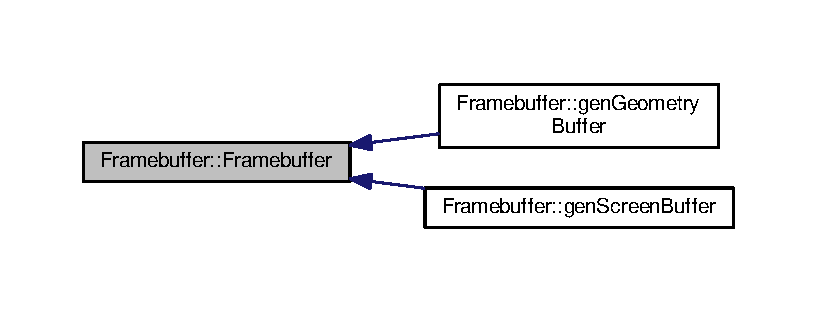
\includegraphics[width=350pt]{class_framebuffer_a4f10f2020d414add1ea0e6553908c86b_icgraph}
\end{center}
\end{figure}


\hypertarget{class_framebuffer_a46ec55ab64b360550afb2de19043852a}{}\index{Framebuffer@{Framebuffer}!Framebuffer@{Framebuffer}}
\index{Framebuffer@{Framebuffer}!Framebuffer@{Framebuffer}}
\subsubsection[{Framebuffer(\+G\+Luint fbo)}]{\setlength{\rightskip}{0pt plus 5cm}Framebuffer\+::\+Framebuffer (
\begin{DoxyParamCaption}
\item[{G\+Luint}]{fbo}
\end{DoxyParamCaption}
)}\label{class_framebuffer_a46ec55ab64b360550afb2de19043852a}
Doesn\textquotesingle{}t create a new I\+D but will delete it in destructor \hypertarget{class_framebuffer_aaed0ae64dc7a0b2762ce74d89913365a}{}\index{Framebuffer@{Framebuffer}!Framebuffer@{Framebuffer}}
\index{Framebuffer@{Framebuffer}!Framebuffer@{Framebuffer}}
\subsubsection[{Framebuffer(int w, int h)}]{\setlength{\rightskip}{0pt plus 5cm}Framebuffer\+::\+Framebuffer (
\begin{DoxyParamCaption}
\item[{int}]{w, }
\item[{int}]{h}
\end{DoxyParamCaption}
)}\label{class_framebuffer_aaed0ae64dc7a0b2762ce74d89913365a}
Constructor 
\begin{DoxyParams}{Parameters}
{\em w} & inital width \\
\hline
{\em h} & initial height \\
\hline
\end{DoxyParams}
\hypertarget{class_framebuffer_a037bf3e17455354d5d907ceea00313dd}{}\index{Framebuffer@{Framebuffer}!````~Framebuffer@{$\sim$\+Framebuffer}}
\index{````~Framebuffer@{$\sim$\+Framebuffer}!Framebuffer@{Framebuffer}}
\subsubsection[{$\sim$\+Framebuffer()}]{\setlength{\rightskip}{0pt plus 5cm}Framebuffer\+::$\sim$\+Framebuffer (
\begin{DoxyParamCaption}
{}
\end{DoxyParamCaption}
)}\label{class_framebuffer_a037bf3e17455354d5d907ceea00313dd}
Deconstructor, deletes all open\+G\+L objects, including the color attachments, associated with the \hyperlink{class_framebuffer}{Framebuffer} 

\subsection{Member Function Documentation}
\hypertarget{class_framebuffer_a167694f148f4de766971234389f04b8a}{}\index{Framebuffer@{Framebuffer}!add\+Attachment@{add\+Attachment}}
\index{add\+Attachment@{add\+Attachment}!Framebuffer@{Framebuffer}}
\subsubsection[{add\+Attachment()}]{\setlength{\rightskip}{0pt plus 5cm}void Framebuffer\+::add\+Attachment (
\begin{DoxyParamCaption}
{}
\end{DoxyParamCaption}
)}\label{class_framebuffer_a167694f148f4de766971234389f04b8a}
Generate a new Color Attachment and add it to the \hyperlink{class_framebuffer}{Framebuffer} 

Here is the call graph for this function\+:\nopagebreak
\begin{figure}[H]
\begin{center}
\leavevmode
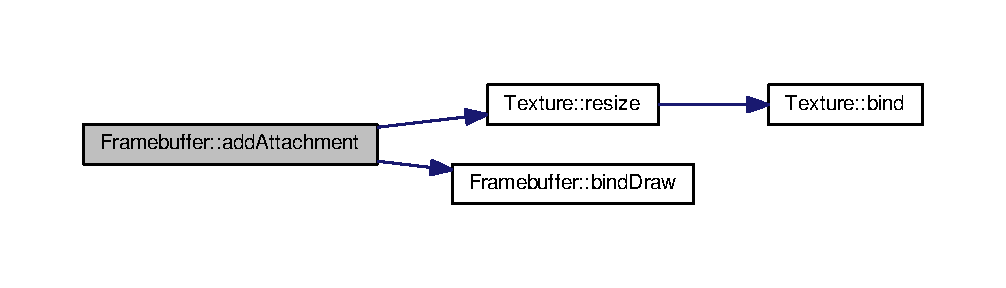
\includegraphics[width=350pt]{class_framebuffer_a167694f148f4de766971234389f04b8a_cgraph}
\end{center}
\end{figure}




Here is the caller graph for this function\+:\nopagebreak
\begin{figure}[H]
\begin{center}
\leavevmode
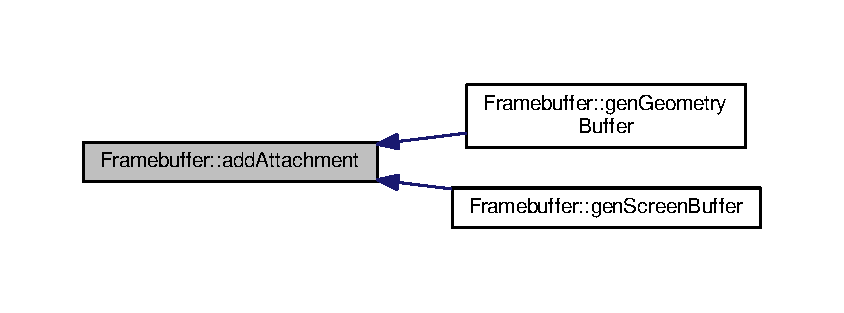
\includegraphics[width=350pt]{class_framebuffer_a167694f148f4de766971234389f04b8a_icgraph}
\end{center}
\end{figure}


\hypertarget{class_framebuffer_a4106324f9cffad333255ce5dab0d4c73}{}\index{Framebuffer@{Framebuffer}!bind\+Draw@{bind\+Draw}}
\index{bind\+Draw@{bind\+Draw}!Framebuffer@{Framebuffer}}
\subsubsection[{bind\+Draw() const }]{\setlength{\rightskip}{0pt plus 5cm}void Framebuffer\+::bind\+Draw (
\begin{DoxyParamCaption}
{}
\end{DoxyParamCaption}
) const}\label{class_framebuffer_a4106324f9cffad333255ce5dab0d4c73}
gl\+Bind\+Framebuffer() wrapper which binds to G\+L\+\_\+\+D\+R\+A\+W\+\_\+\+F\+R\+A\+M\+E\+B\+U\+F\+F\+E\+R aka G\+L\+\_\+\+F\+R\+A\+M\+E\+B\+U\+F\+F\+E\+R 

Here is the caller graph for this function\+:
\nopagebreak
\begin{figure}[H]
\begin{center}
\leavevmode
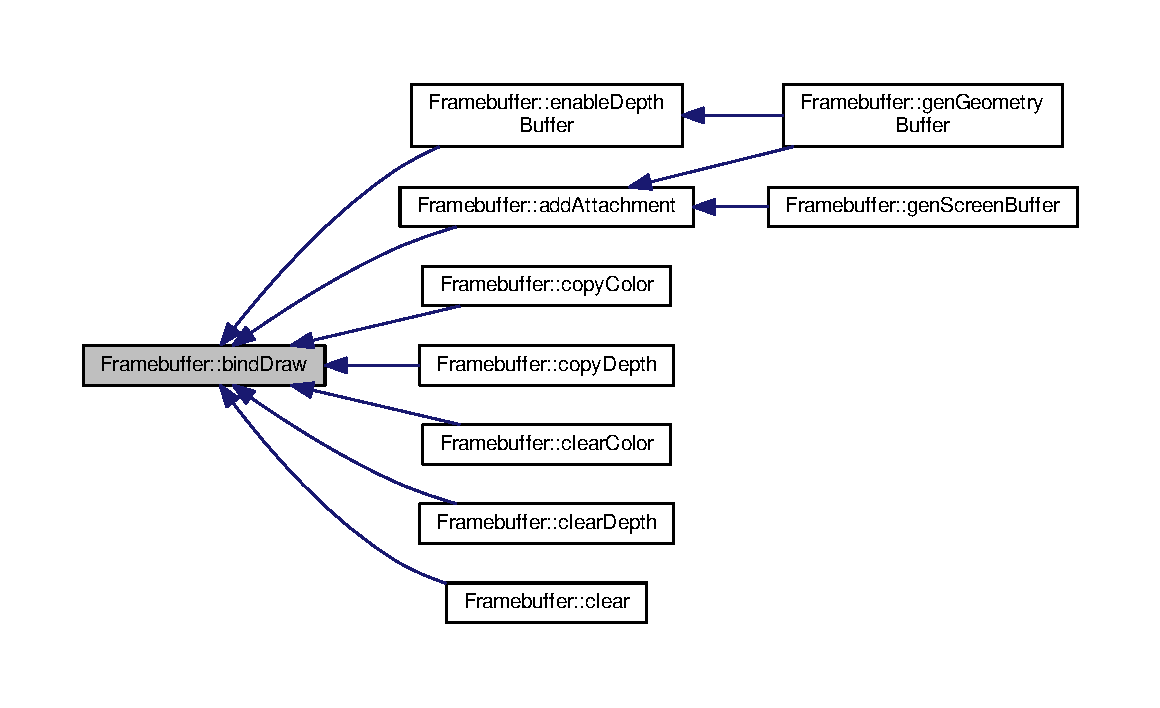
\includegraphics[width=350pt]{class_framebuffer_a4106324f9cffad333255ce5dab0d4c73_icgraph}
\end{center}
\end{figure}


\hypertarget{class_framebuffer_a9f14f58040d7d242f28dad5aff1a5564}{}\index{Framebuffer@{Framebuffer}!bind\+Read@{bind\+Read}}
\index{bind\+Read@{bind\+Read}!Framebuffer@{Framebuffer}}
\subsubsection[{bind\+Read() const }]{\setlength{\rightskip}{0pt plus 5cm}void Framebuffer\+::bind\+Read (
\begin{DoxyParamCaption}
{}
\end{DoxyParamCaption}
) const}\label{class_framebuffer_a9f14f58040d7d242f28dad5aff1a5564}
gl\+Bind\+Framebuffer() wrapper which binds to G\+L\+\_\+\+R\+E\+A\+D\+\_\+\+F\+R\+A\+M\+E\+B\+U\+F\+F\+E\+R 

Here is the caller graph for this function\+:
\nopagebreak
\begin{figure}[H]
\begin{center}
\leavevmode
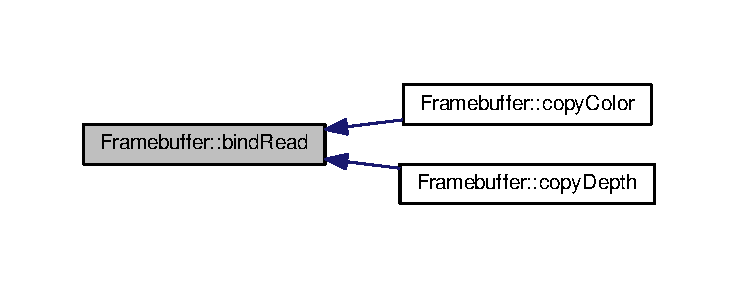
\includegraphics[width=350pt]{class_framebuffer_a9f14f58040d7d242f28dad5aff1a5564_icgraph}
\end{center}
\end{figure}


\hypertarget{class_framebuffer_a29f3edfceab261b122f09a8a1b067b41}{}\index{Framebuffer@{Framebuffer}!clear@{clear}}
\index{clear@{clear}!Framebuffer@{Framebuffer}}
\subsubsection[{clear()}]{\setlength{\rightskip}{0pt plus 5cm}void Framebuffer\+::clear (
\begin{DoxyParamCaption}
{}
\end{DoxyParamCaption}
)}\label{class_framebuffer_a29f3edfceab261b122f09a8a1b067b41}
gl\+Clear() wrapper which clears color and depth 

Here is the call graph for this function\+:\nopagebreak
\begin{figure}[H]
\begin{center}
\leavevmode
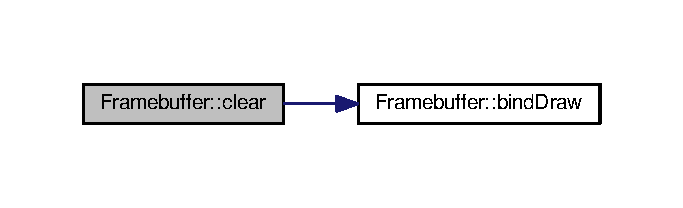
\includegraphics[width=328pt]{class_framebuffer_a29f3edfceab261b122f09a8a1b067b41_cgraph}
\end{center}
\end{figure}


\hypertarget{class_framebuffer_a54aeea0a6f75c104fd974b0743cac55c}{}\index{Framebuffer@{Framebuffer}!clear\+Color@{clear\+Color}}
\index{clear\+Color@{clear\+Color}!Framebuffer@{Framebuffer}}
\subsubsection[{clear\+Color()}]{\setlength{\rightskip}{0pt plus 5cm}void Framebuffer\+::clear\+Color (
\begin{DoxyParamCaption}
{}
\end{DoxyParamCaption}
)}\label{class_framebuffer_a54aeea0a6f75c104fd974b0743cac55c}
gl\+Clear() wrapper which clears color 

Here is the call graph for this function\+:\nopagebreak
\begin{figure}[H]
\begin{center}
\leavevmode
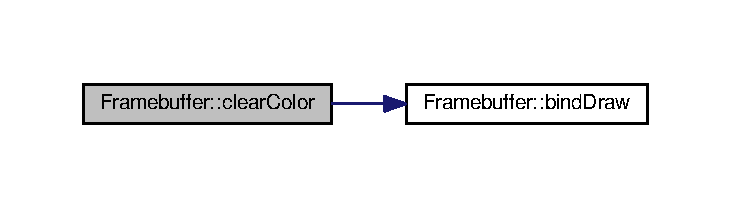
\includegraphics[width=350pt]{class_framebuffer_a54aeea0a6f75c104fd974b0743cac55c_cgraph}
\end{center}
\end{figure}


\hypertarget{class_framebuffer_a01944581e97067094ae7902c43da45ee}{}\index{Framebuffer@{Framebuffer}!clear\+Depth@{clear\+Depth}}
\index{clear\+Depth@{clear\+Depth}!Framebuffer@{Framebuffer}}
\subsubsection[{clear\+Depth()}]{\setlength{\rightskip}{0pt plus 5cm}void Framebuffer\+::clear\+Depth (
\begin{DoxyParamCaption}
{}
\end{DoxyParamCaption}
)}\label{class_framebuffer_a01944581e97067094ae7902c43da45ee}
gl\+Clear() wrapper which clears depth 

Here is the call graph for this function\+:\nopagebreak
\begin{figure}[H]
\begin{center}
\leavevmode
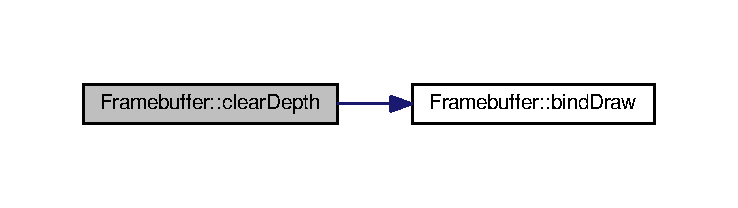
\includegraphics[width=350pt]{class_framebuffer_a01944581e97067094ae7902c43da45ee_cgraph}
\end{center}
\end{figure}


\hypertarget{class_framebuffer_a2182f6f6c725b0efa128a6b5775241e8}{}\index{Framebuffer@{Framebuffer}!copy\+Color@{copy\+Color}}
\index{copy\+Color@{copy\+Color}!Framebuffer@{Framebuffer}}
\subsubsection[{copy\+Color(const Framebuffer \&fb)}]{\setlength{\rightskip}{0pt plus 5cm}void Framebuffer\+::copy\+Color (
\begin{DoxyParamCaption}
\item[{const {\bf Framebuffer} \&}]{fb}
\end{DoxyParamCaption}
)}\label{class_framebuffer_a2182f6f6c725b0efa128a6b5775241e8}
gl\+Blit\+Framebuffer() wrapper which copies color 
\begin{DoxyParams}{Parameters}
{\em fb} & source \hyperlink{class_framebuffer}{Framebuffer} \\
\hline
\end{DoxyParams}


Here is the call graph for this function\+:\nopagebreak
\begin{figure}[H]
\begin{center}
\leavevmode
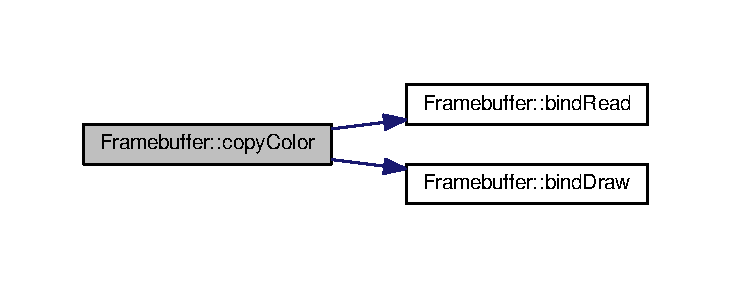
\includegraphics[width=350pt]{class_framebuffer_a2182f6f6c725b0efa128a6b5775241e8_cgraph}
\end{center}
\end{figure}


\hypertarget{class_framebuffer_a3fdff897f598d2c659e251de3c8325da}{}\index{Framebuffer@{Framebuffer}!copy\+Depth@{copy\+Depth}}
\index{copy\+Depth@{copy\+Depth}!Framebuffer@{Framebuffer}}
\subsubsection[{copy\+Depth(const Framebuffer \&fb)}]{\setlength{\rightskip}{0pt plus 5cm}void Framebuffer\+::copy\+Depth (
\begin{DoxyParamCaption}
\item[{const {\bf Framebuffer} \&}]{fb}
\end{DoxyParamCaption}
)}\label{class_framebuffer_a3fdff897f598d2c659e251de3c8325da}
gl\+Blit\+Framebuffer() wrapper which copies depth 
\begin{DoxyParams}{Parameters}
{\em fb} & source \hyperlink{class_framebuffer}{Framebuffer} \\
\hline
\end{DoxyParams}


Here is the call graph for this function\+:\nopagebreak
\begin{figure}[H]
\begin{center}
\leavevmode
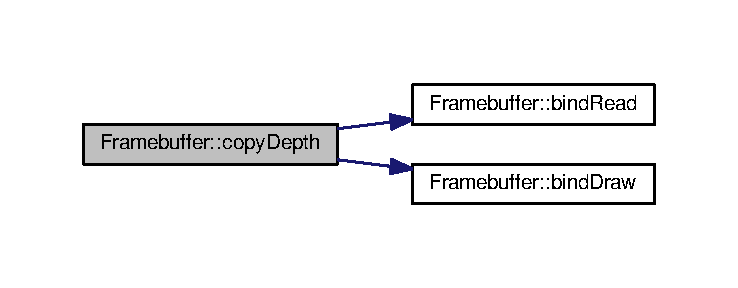
\includegraphics[width=350pt]{class_framebuffer_a3fdff897f598d2c659e251de3c8325da_cgraph}
\end{center}
\end{figure}


\hypertarget{class_framebuffer_a1cc8b67cd13927bfb88b52fe5886d580}{}\index{Framebuffer@{Framebuffer}!enable\+Depth\+Buffer@{enable\+Depth\+Buffer}}
\index{enable\+Depth\+Buffer@{enable\+Depth\+Buffer}!Framebuffer@{Framebuffer}}
\subsubsection[{enable\+Depth\+Buffer(\+G\+Lenum internal\+Format=\+G\+L\+\_\+\+D\+E\+P\+T\+H\+\_\+\+C\+O\+M\+P\+O\+N\+E\+N\+T16)}]{\setlength{\rightskip}{0pt plus 5cm}void Framebuffer\+::enable\+Depth\+Buffer (
\begin{DoxyParamCaption}
\item[{G\+Lenum}]{internal\+Format = {\ttfamily GL\+\_\+DEPTH\+\_\+COMPONENT16}}
\end{DoxyParamCaption}
)}\label{class_framebuffer_a1cc8b67cd13927bfb88b52fe5886d580}
Create Depth Renderbuffer and add it to the Frambuffer 

Here is the call graph for this function\+:\nopagebreak
\begin{figure}[H]
\begin{center}
\leavevmode
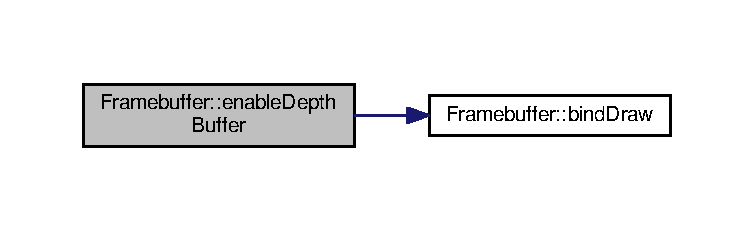
\includegraphics[width=350pt]{class_framebuffer_a1cc8b67cd13927bfb88b52fe5886d580_cgraph}
\end{center}
\end{figure}




Here is the caller graph for this function\+:
\nopagebreak
\begin{figure}[H]
\begin{center}
\leavevmode
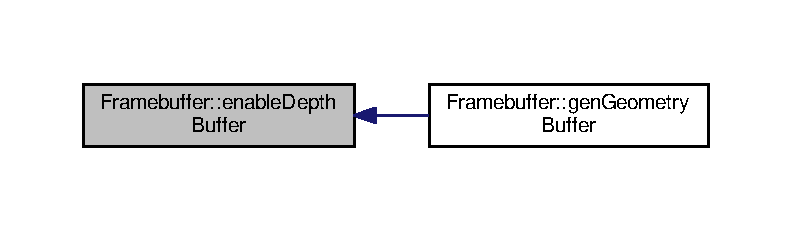
\includegraphics[width=350pt]{class_framebuffer_a1cc8b67cd13927bfb88b52fe5886d580_icgraph}
\end{center}
\end{figure}


\hypertarget{class_framebuffer_add4c1f7b2a3eb1eb007c297b0ac0d88d}{}\index{Framebuffer@{Framebuffer}!gen\+Geometry\+Buffer@{gen\+Geometry\+Buffer}}
\index{gen\+Geometry\+Buffer@{gen\+Geometry\+Buffer}!Framebuffer@{Framebuffer}}
\subsubsection[{gen\+Geometry\+Buffer()}]{\setlength{\rightskip}{0pt plus 5cm}{\bf Framebuffer} $\ast$ Framebuffer\+::gen\+Geometry\+Buffer (
\begin{DoxyParamCaption}
{}
\end{DoxyParamCaption}
)\hspace{0.3cm}{\ttfamily [static]}}\label{class_framebuffer_add4c1f7b2a3eb1eb007c297b0ac0d88d}
Generate a \hyperlink{class_framebuffer}{Framebuffer} with 3 color attachments and depth renderbuffer. attachment 0\+: R\+G\+B\+A16\+F, colors attachment 1\+: R\+G\+B32\+F, positions attachment 2\+: R\+G\+B32\+F, normals \begin{DoxyReturn}{Returns}
Pointer to G\+Buffer which you need to delete 
\end{DoxyReturn}


Here is the call graph for this function\+:\nopagebreak
\begin{figure}[H]
\begin{center}
\leavevmode
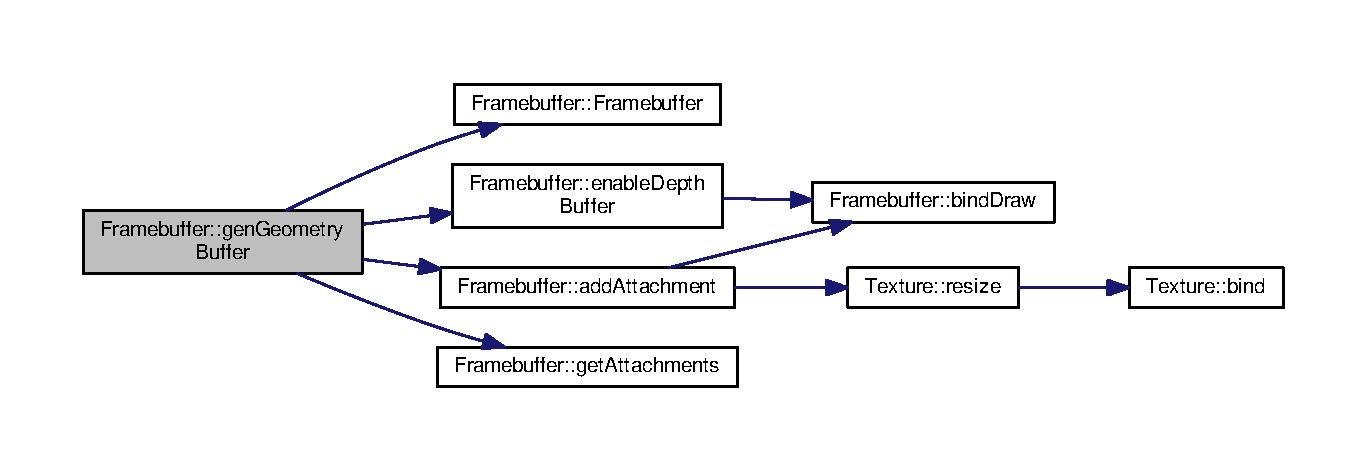
\includegraphics[width=350pt]{class_framebuffer_add4c1f7b2a3eb1eb007c297b0ac0d88d_cgraph}
\end{center}
\end{figure}


\hypertarget{class_framebuffer_a6df15a90817f9f0b364d8a9c2050f481}{}\index{Framebuffer@{Framebuffer}!gen\+Screen\+Buffer@{gen\+Screen\+Buffer}}
\index{gen\+Screen\+Buffer@{gen\+Screen\+Buffer}!Framebuffer@{Framebuffer}}
\subsubsection[{gen\+Screen\+Buffer()}]{\setlength{\rightskip}{0pt plus 5cm}{\bf Framebuffer} $\ast$ Framebuffer\+::gen\+Screen\+Buffer (
\begin{DoxyParamCaption}
{}
\end{DoxyParamCaption}
)\hspace{0.3cm}{\ttfamily [static]}}\label{class_framebuffer_a6df15a90817f9f0b364d8a9c2050f481}
Generate standard \hyperlink{class_framebuffer}{Framebuffer} with no depth and one R\+G\+B color attachment \begin{DoxyReturn}{Returns}
Pointer to Frame\+Buffer which you need to delete 
\end{DoxyReturn}


Here is the call graph for this function\+:\nopagebreak
\begin{figure}[H]
\begin{center}
\leavevmode
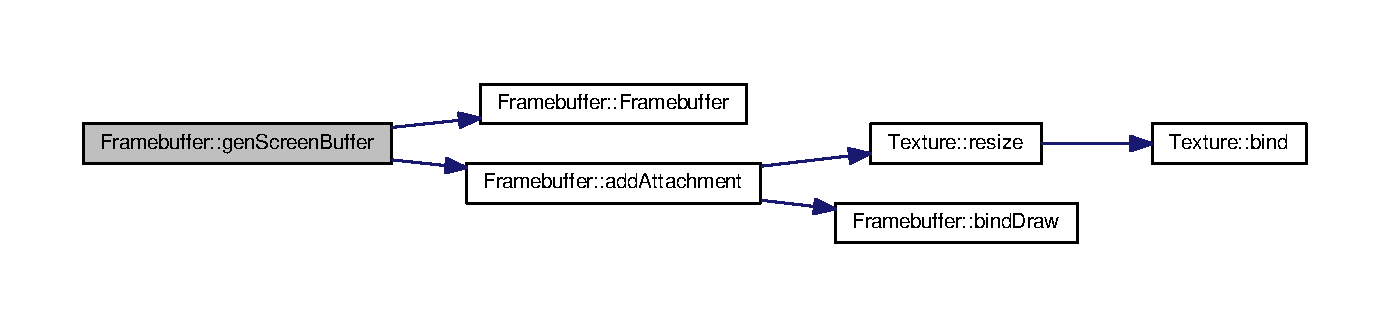
\includegraphics[width=350pt]{class_framebuffer_a6df15a90817f9f0b364d8a9c2050f481_cgraph}
\end{center}
\end{figure}


\hypertarget{class_framebuffer_ae6fe9b975e5a186087fcb53bcfbf7a9d}{}\index{Framebuffer@{Framebuffer}!get\+Active\+Draw@{get\+Active\+Draw}}
\index{get\+Active\+Draw@{get\+Active\+Draw}!Framebuffer@{Framebuffer}}
\subsubsection[{get\+Active\+Draw()}]{\setlength{\rightskip}{0pt plus 5cm}const {\bf Framebuffer} $\ast$ Framebuffer\+::get\+Active\+Draw (
\begin{DoxyParamCaption}
{}
\end{DoxyParamCaption}
)\hspace{0.3cm}{\ttfamily [static]}}\label{class_framebuffer_ae6fe9b975e5a186087fcb53bcfbf7a9d}
Get currently bound drawing \hyperlink{class_framebuffer}{Framebuffer} \hypertarget{class_framebuffer_a0871301296352207df787148de752a21}{}\index{Framebuffer@{Framebuffer}!get\+Active\+Read@{get\+Active\+Read}}
\index{get\+Active\+Read@{get\+Active\+Read}!Framebuffer@{Framebuffer}}
\subsubsection[{get\+Active\+Read()}]{\setlength{\rightskip}{0pt plus 5cm}const {\bf Framebuffer} $\ast$ Framebuffer\+::get\+Active\+Read (
\begin{DoxyParamCaption}
{}
\end{DoxyParamCaption}
)\hspace{0.3cm}{\ttfamily [static]}}\label{class_framebuffer_a0871301296352207df787148de752a21}
Get currently bound reading \hyperlink{class_framebuffer}{Framebuffer} \hypertarget{class_framebuffer_aab2ffec3fc4c6d5efe71e2a8bea64f8b}{}\index{Framebuffer@{Framebuffer}!get\+Attachments@{get\+Attachments}}
\index{get\+Attachments@{get\+Attachments}!Framebuffer@{Framebuffer}}
\subsubsection[{get\+Attachments()}]{\setlength{\rightskip}{0pt plus 5cm}std\+::vector$<$ {\bf Texture} $\ast$ $>$ \& Framebuffer\+::get\+Attachments (
\begin{DoxyParamCaption}
{}
\end{DoxyParamCaption}
)}\label{class_framebuffer_aab2ffec3fc4c6d5efe71e2a8bea64f8b}
Get vector of attached textures 

Here is the caller graph for this function\+:
\nopagebreak
\begin{figure}[H]
\begin{center}
\leavevmode
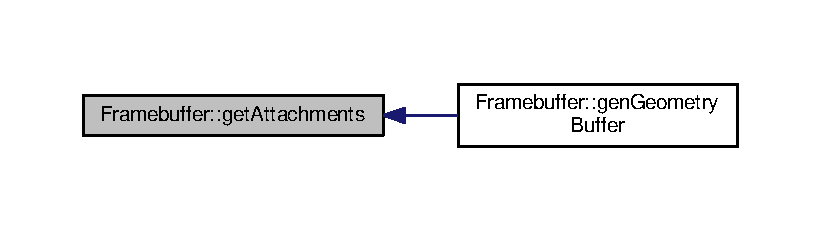
\includegraphics[width=350pt]{class_framebuffer_aab2ffec3fc4c6d5efe71e2a8bea64f8b_icgraph}
\end{center}
\end{figure}


\hypertarget{class_framebuffer_af19335525cae0fb92f20aa46f18d426c}{}\index{Framebuffer@{Framebuffer}!get\+F\+B\+O@{get\+F\+B\+O}}
\index{get\+F\+B\+O@{get\+F\+B\+O}!Framebuffer@{Framebuffer}}
\subsubsection[{get\+F\+B\+O() const }]{\setlength{\rightskip}{0pt plus 5cm}G\+Luint Framebuffer\+::get\+F\+B\+O (
\begin{DoxyParamCaption}
{}
\end{DoxyParamCaption}
) const}\label{class_framebuffer_af19335525cae0fb92f20aa46f18d426c}
Get open\+G\+L I\+D \hypertarget{class_framebuffer_ab1e7b6a5fb21ab0462536f823c97f7d1}{}\index{Framebuffer@{Framebuffer}!get\+Height@{get\+Height}}
\index{get\+Height@{get\+Height}!Framebuffer@{Framebuffer}}
\subsubsection[{get\+Height() const }]{\setlength{\rightskip}{0pt plus 5cm}int Framebuffer\+::get\+Height (
\begin{DoxyParamCaption}
{}
\end{DoxyParamCaption}
) const}\label{class_framebuffer_ab1e7b6a5fb21ab0462536f823c97f7d1}
Get height \hypertarget{class_framebuffer_a7b32671cc35241f0e8a75fe0565003d8}{}\index{Framebuffer@{Framebuffer}!get\+Width@{get\+Width}}
\index{get\+Width@{get\+Width}!Framebuffer@{Framebuffer}}
\subsubsection[{get\+Width() const }]{\setlength{\rightskip}{0pt plus 5cm}int Framebuffer\+::get\+Width (
\begin{DoxyParamCaption}
{}
\end{DoxyParamCaption}
) const}\label{class_framebuffer_a7b32671cc35241f0e8a75fe0565003d8}
Get width \hypertarget{class_framebuffer_a9479ea40d39418a623f64d91b151163f}{}\index{Framebuffer@{Framebuffer}!resize@{resize}}
\index{resize@{resize}!Framebuffer@{Framebuffer}}
\subsubsection[{resize(int w, int h)}]{\setlength{\rightskip}{0pt plus 5cm}void Framebuffer\+::resize (
\begin{DoxyParamCaption}
\item[{int}]{w, }
\item[{int}]{h}
\end{DoxyParamCaption}
)}\label{class_framebuffer_a9479ea40d39418a623f64d91b151163f}
Set the size of the \hyperlink{class_framebuffer}{Framebuffer} and all of its attachments 
\begin{DoxyParams}{Parameters}
{\em w} & the new width \\
\hline
{\em h} & the new height \\
\hline
\end{DoxyParams}


The documentation for this class was generated from the following files\+:\begin{DoxyCompactItemize}
\item 
src/framebuffer.\+h\item 
src/framebuffer.\+cpp\end{DoxyCompactItemize}

\hypertarget{class_height_map}{}\section{Height\+Map Class Reference}
\label{class_height_map}\index{Height\+Map@{Height\+Map}}
\subsection*{Public Member Functions}
\begin{DoxyCompactItemize}
\item 
\hypertarget{class_height_map_a32ace940baafd3dac7228b0949334891}{}{\bfseries Height\+Map} (const \hyperlink{class_height_map}{Height\+Map} \&copy)\label{class_height_map_a32ace940baafd3dac7228b0949334891}

\item 
\hypertarget{class_height_map_a7992f55c4c5c7fb453f89beb892a4fb8}{}{\bfseries Height\+Map} (size\+\_\+t w, size\+\_\+t h)\label{class_height_map_a7992f55c4c5c7fb453f89beb892a4fb8}

\end{DoxyCompactItemize}
\subsection*{Static Public Member Functions}
\begin{DoxyCompactItemize}
\item 
\hypertarget{class_height_map_acd1d7ed04f2e2ad0411378555c1b3c36}{}static \hyperlink{class_height_map}{Height\+Map} {\bfseries gen\+Random} (unsigned int pow)\label{class_height_map_acd1d7ed04f2e2ad0411378555c1b3c36}

\end{DoxyCompactItemize}
\subsection*{Public Attributes}
\begin{DoxyCompactItemize}
\item 
\hypertarget{class_height_map_a03f2518009888c748d122b1771dd0b8b}{}G\+Luint {\bfseries texture}\label{class_height_map_a03f2518009888c748d122b1771dd0b8b}

\item 
\hypertarget{class_height_map_aca9c8c47bce2ea134dd7206bdeef0040}{}double $\ast$$\ast$ {\bfseries data}\label{class_height_map_aca9c8c47bce2ea134dd7206bdeef0040}

\item 
\hypertarget{class_height_map_a674095275a539d9cbeffe7ba0ae36bcc}{}size\+\_\+t {\bfseries width}\label{class_height_map_a674095275a539d9cbeffe7ba0ae36bcc}

\item 
\hypertarget{class_height_map_a6640eb96152cb578ebc107e29207a35a}{}size\+\_\+t {\bfseries height}\label{class_height_map_a6640eb96152cb578ebc107e29207a35a}

\end{DoxyCompactItemize}


The documentation for this class was generated from the following files\+:\begin{DoxyCompactItemize}
\item 
src/terrain.\+h\item 
src/terrain.\+cpp\end{DoxyCompactItemize}

\hypertarget{class_lighting}{}\section{Lighting Class Reference}
\label{class_lighting}\index{Lighting@{Lighting}}


Inheritance diagram for Lighting\+:\nopagebreak
\begin{figure}[H]
\begin{center}
\leavevmode
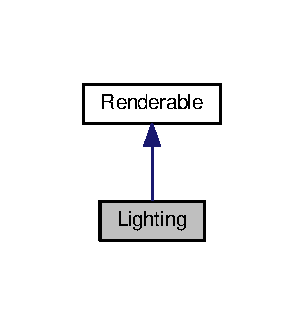
\includegraphics[width=146pt]{class_lighting__inherit__graph}
\end{center}
\end{figure}


Collaboration diagram for Lighting\+:\nopagebreak
\begin{figure}[H]
\begin{center}
\leavevmode
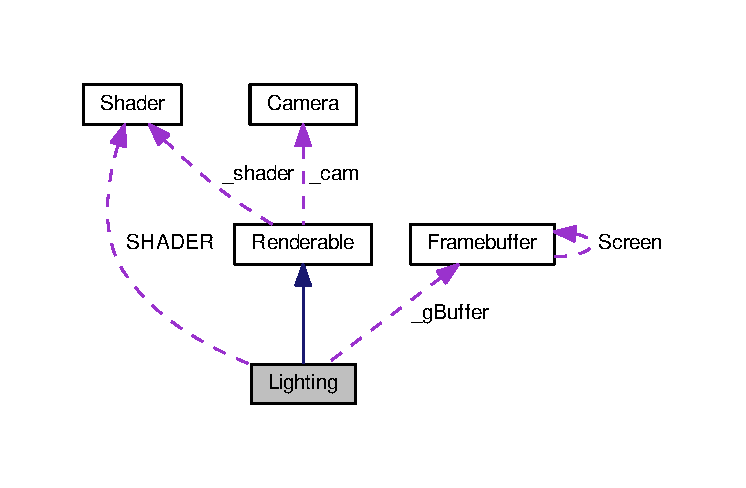
\includegraphics[width=350pt]{class_lighting__coll__graph}
\end{center}
\end{figure}
\subsection*{Public Member Functions}
\begin{DoxyCompactItemize}
\item 
\hypertarget{class_lighting_ac786f1b90379f996f8d99e1e4bcd9e6f}{}{\bfseries Lighting} (\hyperlink{class_perspective_camera}{Perspective\+Camera} $\ast$cam, \hyperlink{class_framebuffer}{Framebuffer} $\ast$g\+Buffer)\label{class_lighting_ac786f1b90379f996f8d99e1e4bcd9e6f}

\item 
\hypertarget{class_lighting_a139c84b1a180648b41694b47f281981b}{}virtual void {\bfseries render} ()\label{class_lighting_a139c84b1a180648b41694b47f281981b}

\item 
\hypertarget{class_lighting_a124e1e665b5907faf9c52bd851f1a417}{}void {\bfseries add\+Point\+Light} (\hyperlink{class_point_light}{Point\+Light} $\ast$light)\label{class_lighting_a124e1e665b5907faf9c52bd851f1a417}

\item 
\hypertarget{class_lighting_a7d78793f7c5e3eb05b222309b7d8c617}{}void {\bfseries remove\+Point\+Light} (\hyperlink{class_point_light}{Point\+Light} $\ast$light)\label{class_lighting_a7d78793f7c5e3eb05b222309b7d8c617}

\end{DoxyCompactItemize}
\subsection*{Static Public Attributes}
\begin{DoxyCompactItemize}
\item 
\hypertarget{class_lighting_add6b069bd3d0f36eee753fe3470fe22d}{}static \hyperlink{class_shader}{Shader} $\ast$ {\bfseries S\+H\+A\+D\+E\+R} = 0\label{class_lighting_add6b069bd3d0f36eee753fe3470fe22d}

\end{DoxyCompactItemize}
\subsection*{Protected Attributes}
\begin{DoxyCompactItemize}
\item 
\hypertarget{class_lighting_a85e99efa5af1df4462e6e63c7886701d}{}\hyperlink{class_framebuffer}{Framebuffer} $\ast$ {\bfseries \+\_\+g\+Buffer}\label{class_lighting_a85e99efa5af1df4462e6e63c7886701d}

\item 
\hypertarget{class_lighting_a05e11ba57df9a979c8913276eb4c2fe0}{}std\+::vector$<$ \hyperlink{class_attribute}{Attribute} $>$ {\bfseries \+\_\+attributes}\label{class_lighting_a05e11ba57df9a979c8913276eb4c2fe0}

\item 
\hypertarget{class_lighting_adcc02d75999339a316e9ff9c909ba0ee}{}std\+::vector$<$ \hyperlink{class_point_light}{Point\+Light} $\ast$ $>$ {\bfseries \+\_\+lights}\label{class_lighting_adcc02d75999339a316e9ff9c909ba0ee}

\item 
\hypertarget{class_lighting_ad2ad50701ec4fc496bf786a1c64f6442}{}glm\+::vec3 {\bfseries \+\_\+ambient}\label{class_lighting_ad2ad50701ec4fc496bf786a1c64f6442}

\item 
\hypertarget{class_lighting_acd98b5fd27f0267fd4106c8749e7c1f0}{}glm\+::vec3 {\bfseries \+\_\+sun\+Dir}\label{class_lighting_acd98b5fd27f0267fd4106c8749e7c1f0}

\item 
\hypertarget{class_lighting_ae1fb12c3c1bff3ebe4224b5417860e7f}{}glm\+::vec3 {\bfseries \+\_\+sun\+Diffuse}\label{class_lighting_ae1fb12c3c1bff3ebe4224b5417860e7f}

\item 
\hypertarget{class_lighting_a149d381c877a39f01bfdab7f6842001c}{}glm\+::vec3 {\bfseries \+\_\+sun\+Specular}\label{class_lighting_a149d381c877a39f01bfdab7f6842001c}

\end{DoxyCompactItemize}


The documentation for this class was generated from the following files\+:\begin{DoxyCompactItemize}
\item 
src/lighting.\+h\item 
src/lighting.\+cpp\end{DoxyCompactItemize}

\hypertarget{class_light_well}{}\section{Light\+Well Class Reference}
\label{class_light_well}\index{Light\+Well@{Light\+Well}}


Inheritance diagram for Light\+Well\+:\nopagebreak
\begin{figure}[H]
\begin{center}
\leavevmode
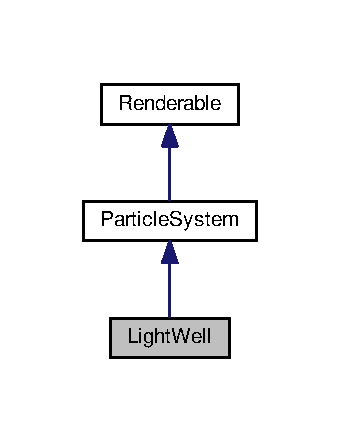
\includegraphics[width=163pt]{class_light_well__inherit__graph}
\end{center}
\end{figure}


Collaboration diagram for Light\+Well\+:\nopagebreak
\begin{figure}[H]
\begin{center}
\leavevmode
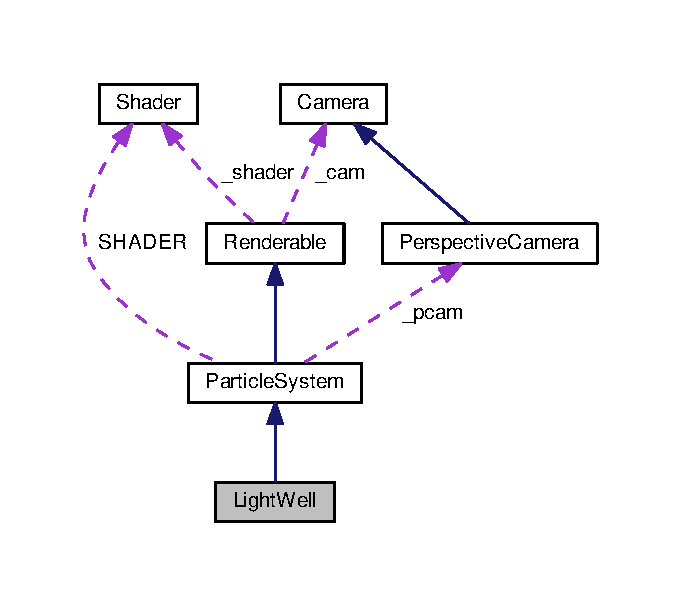
\includegraphics[width=327pt]{class_light_well__coll__graph}
\end{center}
\end{figure}
\subsection*{Public Member Functions}
\begin{DoxyCompactItemize}
\item 
\hypertarget{class_light_well_a211419be5b7ea554fc5b92af2e5fbf1b}{}{\bfseries Light\+Well} (\hyperlink{class_perspective_camera}{Perspective\+Camera} $\ast$cam, glm\+::vec3 pos)\label{class_light_well_a211419be5b7ea554fc5b92af2e5fbf1b}

\item 
\hypertarget{class_light_well_abeca4d5eb016e860bc73910883abd79b}{}void {\bfseries spawn\+Particle} ()\label{class_light_well_abeca4d5eb016e860bc73910883abd79b}

\item 
\hypertarget{class_light_well_a2ef68e3a0a2da1f7f8d9f0f329f53348}{}virtual void {\bfseries step} (double dt)\label{class_light_well_a2ef68e3a0a2da1f7f8d9f0f329f53348}

\end{DoxyCompactItemize}
\subsection*{Protected Attributes}
\begin{DoxyCompactItemize}
\item 
\hypertarget{class_light_well_a90ba1983609cbb3c483d8a023a4bef02}{}glm\+::vec3 {\bfseries \+\_\+pos}\label{class_light_well_a90ba1983609cbb3c483d8a023a4bef02}

\end{DoxyCompactItemize}
\subsection*{Additional Inherited Members}


The documentation for this class was generated from the following files\+:\begin{DoxyCompactItemize}
\item 
src/particle.\+h\item 
src/particle.\+cpp\end{DoxyCompactItemize}

\hypertarget{class_mesh}{}\section{Mesh Class Reference}
\label{class_mesh}\index{Mesh@{Mesh}}


Inheritance diagram for Mesh\+:\nopagebreak
\begin{figure}[H]
\begin{center}
\leavevmode
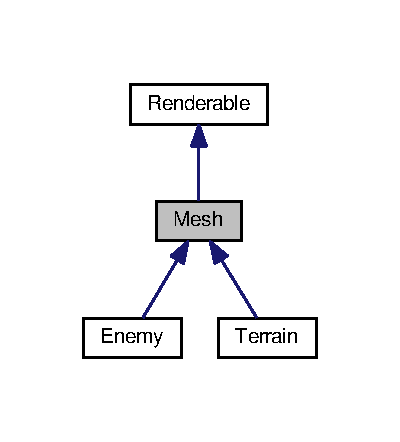
\includegraphics[width=192pt]{class_mesh__inherit__graph}
\end{center}
\end{figure}


Collaboration diagram for Mesh\+:\nopagebreak
\begin{figure}[H]
\begin{center}
\leavevmode
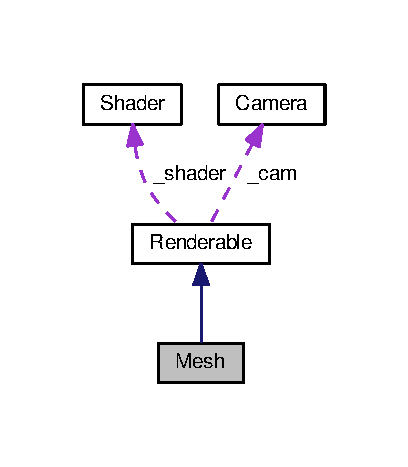
\includegraphics[width=196pt]{class_mesh__coll__graph}
\end{center}
\end{figure}
\subsection*{Public Member Functions}
\begin{DoxyCompactItemize}
\item 
\hypertarget{class_mesh_ace06807c618667a649c0d7e59bddde6b}{}{\bfseries Mesh} (\hyperlink{class_camera}{Camera} $\ast$cam, \hyperlink{class_mesh_data}{Mesh\+Data} $\ast$data, G\+Luint texture)\label{class_mesh_ace06807c618667a649c0d7e59bddde6b}

\item 
\hypertarget{class_mesh_aa196429f3e87ecd53e8770ba979222f4}{}virtual void {\bfseries render} ()\label{class_mesh_aa196429f3e87ecd53e8770ba979222f4}

\item 
\hypertarget{class_mesh_a363f6809aa3269a7021a68421f1bb160}{}void {\bfseries toggle\+Wireframe} ()\label{class_mesh_a363f6809aa3269a7021a68421f1bb160}

\end{DoxyCompactItemize}
\subsection*{Protected Attributes}
\begin{DoxyCompactItemize}
\item 
\hypertarget{class_mesh_a22f29d6780b3da1f252d8f3bb99b0be2}{}G\+Luint {\bfseries \+\_\+texture}\label{class_mesh_a22f29d6780b3da1f252d8f3bb99b0be2}

\item 
\hypertarget{class_mesh_ad9fc3eaca88e3ebcde82c16476517e92}{}bool {\bfseries \+\_\+wireframe}\label{class_mesh_ad9fc3eaca88e3ebcde82c16476517e92}

\item 
\hypertarget{class_mesh_a3d161b2b2e8731ffe4d6a24fe3730662}{}glm\+::vec4 {\bfseries \+\_\+diffuse\+Color}\label{class_mesh_a3d161b2b2e8731ffe4d6a24fe3730662}

\item 
\hypertarget{class_mesh_a3f694254f04807332a6edfd2558ab115}{}glm\+::mat4 {\bfseries \+\_\+model}\label{class_mesh_a3f694254f04807332a6edfd2558ab115}

\end{DoxyCompactItemize}


The documentation for this class was generated from the following files\+:\begin{DoxyCompactItemize}
\item 
src/mesh.\+h\item 
src/mesh.\+cpp\end{DoxyCompactItemize}

\hypertarget{class_mesh_data}{}\section{Mesh\+Data Class Reference}
\label{class_mesh_data}\index{Mesh\+Data@{Mesh\+Data}}


{\ttfamily \#include $<$mesh.\+h$>$}



Collaboration diagram for Mesh\+Data\+:\nopagebreak
\begin{figure}[H]
\begin{center}
\leavevmode
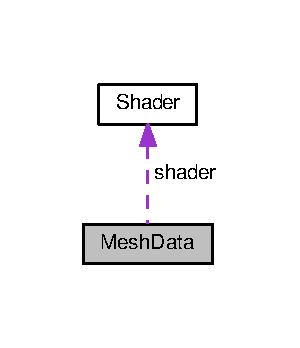
\includegraphics[width=144pt]{class_mesh_data__coll__graph}
\end{center}
\end{figure}
\subsection*{Public Member Functions}
\begin{DoxyCompactItemize}
\item 
\hypertarget{class_mesh_data_a5a1e14216ee9b2162d998f2c2612b94e}{}{\bfseries Mesh\+Data} (G\+Lfloat $\ast$vertices, G\+Lfloat $\ast$normals, G\+Lfloat $\ast$uvs, size\+\_\+t verts, unsigned short $\ast$indices, size\+\_\+t elements)\label{class_mesh_data_a5a1e14216ee9b2162d998f2c2612b94e}

\end{DoxyCompactItemize}
\subsection*{Static Public Member Functions}
\begin{DoxyCompactItemize}
\item 
\hypertarget{class_mesh_data_a1c7e76f9be2d77165d0efa8a1f9e3529}{}static \hyperlink{class_mesh_data}{Mesh\+Data} {\bfseries gen\+Ico\+Sphere} ()\label{class_mesh_data_a1c7e76f9be2d77165d0efa8a1f9e3529}

\item 
\hypertarget{class_mesh_data_a7633222ba1b61c6898a495348c8558fb}{}static \hyperlink{class_mesh_data}{Mesh\+Data} {\bfseries gen\+Cube} ()\label{class_mesh_data_a7633222ba1b61c6898a495348c8558fb}

\end{DoxyCompactItemize}
\subsection*{Public Attributes}
\begin{DoxyCompactItemize}
\item 
\hypertarget{class_mesh_data_a1fe829b1f1fbc268824cbdf883a78093}{}size\+\_\+t {\bfseries elements}\label{class_mesh_data_a1fe829b1f1fbc268824cbdf883a78093}

\item 
\hypertarget{class_mesh_data_a78e8a966051cd6c5c0460074cac8fd89}{}std\+::vector$<$ \hyperlink{class_attribute}{Attribute} $>$ {\bfseries attributes}\label{class_mesh_data_a78e8a966051cd6c5c0460074cac8fd89}

\item 
\hypertarget{class_mesh_data_a99f16e148d7e476a6bfad9b8b12c9c75}{}G\+Luint {\bfseries index\+Buffer}\label{class_mesh_data_a99f16e148d7e476a6bfad9b8b12c9c75}

\item 
\hypertarget{class_mesh_data_afc5b228a665295bd97ec308367d368d4}{}\hyperlink{class_shader}{Shader} $\ast$ {\bfseries shader}\label{class_mesh_data_afc5b228a665295bd97ec308367d368d4}

\item 
\hypertarget{class_mesh_data_af210d554df28e667ca61e5afa235215b}{}G\+Lenum {\bfseries mode}\label{class_mesh_data_af210d554df28e667ca61e5afa235215b}

\end{DoxyCompactItemize}


\subsection{Detailed Description}
represents \hyperlink{class_mesh}{Mesh} Resources stored on G\+P\+U 

The documentation for this class was generated from the following files\+:\begin{DoxyCompactItemize}
\item 
src/mesh.\+h\item 
src/mesh.\+cpp\end{DoxyCompactItemize}

\hypertarget{class_particle}{}\section{Particle Class Reference}
\label{class_particle}\index{Particle@{Particle}}


Collaboration diagram for Particle\+:\nopagebreak
\begin{figure}[H]
\begin{center}
\leavevmode
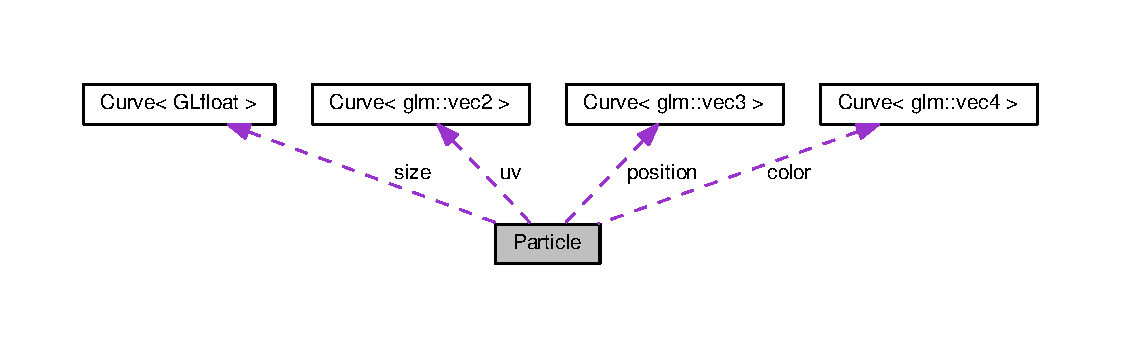
\includegraphics[width=350pt]{class_particle__coll__graph}
\end{center}
\end{figure}
\subsection*{Public Member Functions}
\begin{DoxyCompactItemize}
\item 
\hypertarget{class_particle_a4d305fe8deed42f61776100729b6298e}{}virtual void {\bfseries step} (double dt)\label{class_particle_a4d305fe8deed42f61776100729b6298e}

\end{DoxyCompactItemize}
\subsection*{Public Attributes}
\begin{DoxyCompactItemize}
\item 
\hypertarget{class_particle_a31b8e2a4c6f8c10ea00878599b7d40b6}{}\hyperlink{class_curve}{Curve}$<$ glm\+::vec3 $>$ {\bfseries position}\label{class_particle_a31b8e2a4c6f8c10ea00878599b7d40b6}

\item 
\hypertarget{class_particle_a819fdee7e19d9b4a804bd65c3b1ed10a}{}\hyperlink{class_curve}{Curve}$<$ glm\+::vec2 $>$ \hyperlink{class_particle_a819fdee7e19d9b4a804bd65c3b1ed10a}{uv}\label{class_particle_a819fdee7e19d9b4a804bd65c3b1ed10a}

\begin{DoxyCompactList}\small\item\em for texture animation \end{DoxyCompactList}\item 
\hypertarget{class_particle_a6b07b59be5260cf2694ecb02165ad7bd}{}\hyperlink{class_curve}{Curve}$<$ glm\+::vec4 $>$ {\bfseries color}\label{class_particle_a6b07b59be5260cf2694ecb02165ad7bd}

\item 
\hypertarget{class_particle_aa023368080fd9cb8b533cc5124452c7e}{}\hyperlink{class_curve}{Curve}$<$ G\+Lfloat $>$ {\bfseries size}\label{class_particle_aa023368080fd9cb8b533cc5124452c7e}

\item 
\hypertarget{class_particle_a1760a331eebb54cbdd6ca280439a36c8}{}float {\bfseries life}\label{class_particle_a1760a331eebb54cbdd6ca280439a36c8}

\end{DoxyCompactItemize}


The documentation for this class was generated from the following file\+:\begin{DoxyCompactItemize}
\item 
src/particle.\+h\end{DoxyCompactItemize}

\hypertarget{class_particle_system}{}\section{Particle\+System Class Reference}
\label{class_particle_system}\index{Particle\+System@{Particle\+System}}


Inheritance diagram for Particle\+System\+:\nopagebreak
\begin{figure}[H]
\begin{center}
\leavevmode
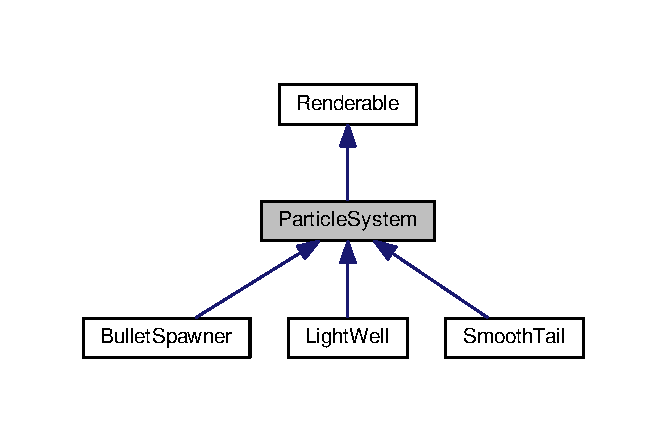
\includegraphics[width=320pt]{class_particle_system__inherit__graph}
\end{center}
\end{figure}


Collaboration diagram for Particle\+System\+:\nopagebreak
\begin{figure}[H]
\begin{center}
\leavevmode
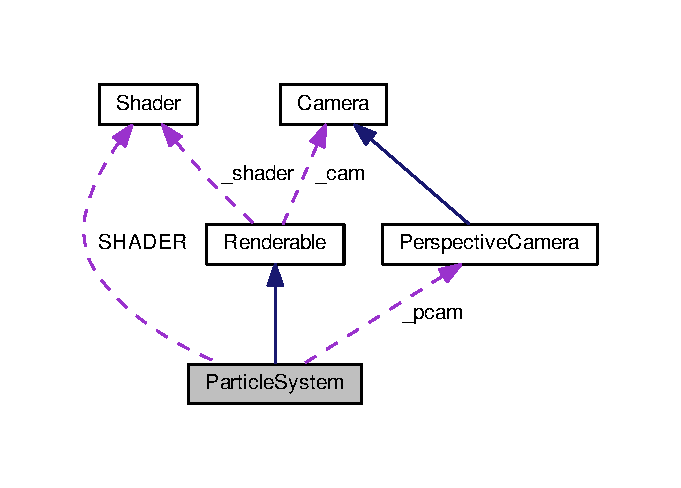
\includegraphics[width=327pt]{class_particle_system__coll__graph}
\end{center}
\end{figure}
\subsection*{Public Types}
\begin{DoxyCompactItemize}
\item 
\hypertarget{class_particle_system_a0cb971f2e53dbb81558ff82bef0e7ba5}{}enum {\bfseries Buffer\+Index} \{ {\bfseries P\+O\+S\+I\+T\+I\+O\+N}, 
{\bfseries C\+O\+L\+O\+R}, 
{\bfseries U\+V}, 
{\bfseries S\+I\+Z\+E}
 \}\label{class_particle_system_a0cb971f2e53dbb81558ff82bef0e7ba5}

\end{DoxyCompactItemize}
\subsection*{Public Member Functions}
\begin{DoxyCompactItemize}
\item 
\hypertarget{class_particle_system_aec4b7b019239eea443697b25b1723ae8}{}{\bfseries Particle\+System} (\hyperlink{class_perspective_camera}{Perspective\+Camera} $\ast$cam, G\+Luint texture)\label{class_particle_system_aec4b7b019239eea443697b25b1723ae8}

\item 
\hypertarget{class_particle_system_a5d76bedc89cba3a443b458a6c142b5a6}{}virtual void {\bfseries step} (double dt)\label{class_particle_system_a5d76bedc89cba3a443b458a6c142b5a6}

\item 
\hypertarget{class_particle_system_af2ec9e0fe49695569a9524f6a2238e6f}{}virtual void {\bfseries render} ()\label{class_particle_system_af2ec9e0fe49695569a9524f6a2238e6f}

\end{DoxyCompactItemize}
\subsection*{Static Public Attributes}
\begin{DoxyCompactItemize}
\item 
\hypertarget{class_particle_system_a4161327867c61aaa755895c90693620c}{}static \hyperlink{class_shader}{Shader} $\ast$ {\bfseries S\+H\+A\+D\+E\+R} = 0\label{class_particle_system_a4161327867c61aaa755895c90693620c}

\end{DoxyCompactItemize}
\subsection*{Protected Attributes}
\begin{DoxyCompactItemize}
\item 
\hypertarget{class_particle_system_a5c5e894d64b153f888e59bd888df6346}{}std\+::vector$<$ \hyperlink{class_particle}{Particle} $>$ {\bfseries \+\_\+particles}\label{class_particle_system_a5c5e894d64b153f888e59bd888df6346}

\item 
\hypertarget{class_particle_system_a6c6c5a7616e412278a798d912d0402b4}{}\hyperlink{class_perspective_camera}{Perspective\+Camera} $\ast$ {\bfseries \+\_\+pcam}\label{class_particle_system_a6c6c5a7616e412278a798d912d0402b4}

\end{DoxyCompactItemize}


The documentation for this class was generated from the following files\+:\begin{DoxyCompactItemize}
\item 
src/particle.\+h\item 
src/particle.\+cpp\end{DoxyCompactItemize}

\hypertarget{class_perspective_camera}{}\section{Perspective\+Camera Class Reference}
\label{class_perspective_camera}\index{Perspective\+Camera@{Perspective\+Camera}}


Inheritance diagram for Perspective\+Camera\+:\nopagebreak
\begin{figure}[H]
\begin{center}
\leavevmode
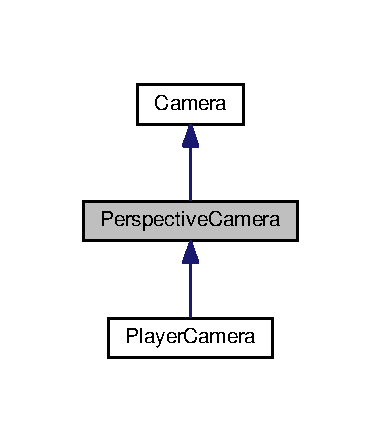
\includegraphics[width=183pt]{class_perspective_camera__inherit__graph}
\end{center}
\end{figure}


Collaboration diagram for Perspective\+Camera\+:\nopagebreak
\begin{figure}[H]
\begin{center}
\leavevmode
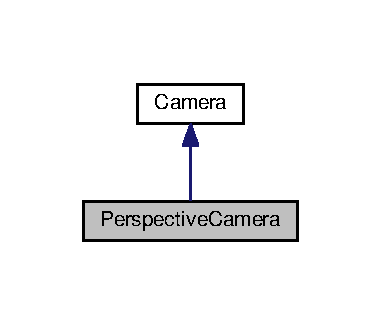
\includegraphics[width=183pt]{class_perspective_camera__coll__graph}
\end{center}
\end{figure}
\subsection*{Public Member Functions}
\begin{DoxyCompactItemize}
\item 
\hypertarget{class_perspective_camera_abd6326664a8e88335c5de79365a1ea15}{}{\bfseries Perspective\+Camera} (float fov, float aspect, float near, float far)\label{class_perspective_camera_abd6326664a8e88335c5de79365a1ea15}

\item 
\hypertarget{class_perspective_camera_ac54590aa7444d2bd2bf4b34b6ef45266}{}virtual void {\bfseries set\+Uniforms} (\hyperlink{class_shader}{Shader} $\ast$shader) const \label{class_perspective_camera_ac54590aa7444d2bd2bf4b34b6ef45266}

\item 
\hypertarget{class_perspective_camera_a5793e6291d90811a6743cac10ae6b0f1}{}void {\bfseries on\+Resize} (int width, int height)\label{class_perspective_camera_a5793e6291d90811a6743cac10ae6b0f1}

\item 
\hypertarget{class_perspective_camera_a36fa85a3f46042dbaf5819b7388b341a}{}glm\+::vec3 {\bfseries get\+Position} () const \label{class_perspective_camera_a36fa85a3f46042dbaf5819b7388b341a}

\item 
\hypertarget{class_perspective_camera_acfac6859cf992701454cb802ffb45796}{}void {\bfseries set\+Position} (const glm\+::vec3 \&eye)\label{class_perspective_camera_acfac6859cf992701454cb802ffb45796}

\item 
\hypertarget{class_perspective_camera_a66f7d8ec9370c792bee1a7c686e0e417}{}void {\bfseries translate} (const glm\+::vec3 \&t)\label{class_perspective_camera_a66f7d8ec9370c792bee1a7c686e0e417}

\item 
\hypertarget{class_perspective_camera_abb05342b409ac950b411e877af5e30f1}{}float {\bfseries get\+Angle\+Y} () const \label{class_perspective_camera_abb05342b409ac950b411e877af5e30f1}

\item 
\hypertarget{class_perspective_camera_a6c466eb6fb577bc67a1a27d40ec93fcf}{}void {\bfseries set\+Angle\+Y} (const float \&a)\label{class_perspective_camera_a6c466eb6fb577bc67a1a27d40ec93fcf}

\item 
\hypertarget{class_perspective_camera_ac3b176a18e12c0927350d3c833e43943}{}void {\bfseries turn\+Y} (const float \&a)\label{class_perspective_camera_ac3b176a18e12c0927350d3c833e43943}

\item 
\hypertarget{class_perspective_camera_a05fc504e191d0ab3abd0ef8189a19e1f}{}float {\bfseries get\+Angle\+X} () const \label{class_perspective_camera_a05fc504e191d0ab3abd0ef8189a19e1f}

\item 
\hypertarget{class_perspective_camera_a6af5d666cd398e375e90ac06364d3545}{}void {\bfseries set\+Angle\+X} (const float \&a)\label{class_perspective_camera_a6af5d666cd398e375e90ac06364d3545}

\item 
\hypertarget{class_perspective_camera_a6bbd0338716891b778c5ce70f1f5fdda}{}void {\bfseries turn\+X} (const float \&a)\label{class_perspective_camera_a6bbd0338716891b778c5ce70f1f5fdda}

\item 
\hypertarget{class_perspective_camera_aa178b372867ae7fa837d83ed506f1f36}{}glm\+::mat4 {\bfseries get\+View} () const \label{class_perspective_camera_aa178b372867ae7fa837d83ed506f1f36}

\end{DoxyCompactItemize}
\subsection*{Static Public Attributes}
\begin{DoxyCompactItemize}
\item 
\hypertarget{class_perspective_camera_a6f9a19c4ebd1f9037707bae4ddba2249}{}static const std\+::string {\bfseries P\+R\+O\+J\+\_\+\+U\+N\+I\+F\+O\+R\+M\+\_\+\+S\+T\+R} = \char`\"{}proj\char`\"{}\label{class_perspective_camera_a6f9a19c4ebd1f9037707bae4ddba2249}

\item 
\hypertarget{class_perspective_camera_a97517e41a2a0298b6d832a2fc7fb205b}{}static const std\+::string {\bfseries V\+I\+E\+W\+\_\+\+U\+N\+I\+F\+O\+R\+M\+\_\+\+S\+T\+R} = \char`\"{}view\char`\"{}\label{class_perspective_camera_a97517e41a2a0298b6d832a2fc7fb205b}

\end{DoxyCompactItemize}
\subsection*{Protected Member Functions}
\begin{DoxyCompactItemize}
\item 
\hypertarget{class_perspective_camera_a1ede24481c69a76465f25a5ac920c1be}{}void {\bfseries update\+View} ()\label{class_perspective_camera_a1ede24481c69a76465f25a5ac920c1be}

\end{DoxyCompactItemize}
\subsection*{Protected Attributes}
\begin{DoxyCompactItemize}
\item 
\hypertarget{class_perspective_camera_abd8e00fd34a5b51b431fb8d32196fe20}{}glm\+::vec3 {\bfseries \+\_\+eye}\label{class_perspective_camera_abd8e00fd34a5b51b431fb8d32196fe20}

\item 
\hypertarget{class_perspective_camera_a789547758df18f7fdc872faf871d085f}{}float \hyperlink{class_perspective_camera_a789547758df18f7fdc872faf871d085f}{\+\_\+angle\+X}\label{class_perspective_camera_a789547758df18f7fdc872faf871d085f}

\begin{DoxyCompactList}\small\item\em angle around X axis \end{DoxyCompactList}\item 
\hypertarget{class_perspective_camera_a09566695cfe277257cde24cb917e9328}{}float \hyperlink{class_perspective_camera_a09566695cfe277257cde24cb917e9328}{\+\_\+angle\+Y}\label{class_perspective_camera_a09566695cfe277257cde24cb917e9328}

\begin{DoxyCompactList}\small\item\em angle around Y axis \end{DoxyCompactList}\end{DoxyCompactItemize}


The documentation for this class was generated from the following files\+:\begin{DoxyCompactItemize}
\item 
src/camera.\+h\item 
src/camera.\+cpp\end{DoxyCompactItemize}

\hypertarget{class_player_camera}{}\section{Player\+Camera Class Reference}
\label{class_player_camera}\index{Player\+Camera@{Player\+Camera}}


Inheritance diagram for Player\+Camera\+:\nopagebreak
\begin{figure}[H]
\begin{center}
\leavevmode
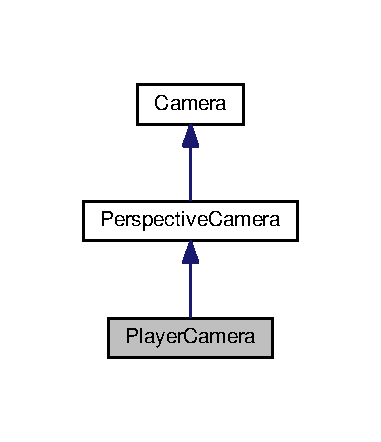
\includegraphics[width=183pt]{class_player_camera__inherit__graph}
\end{center}
\end{figure}


Collaboration diagram for Player\+Camera\+:\nopagebreak
\begin{figure}[H]
\begin{center}
\leavevmode
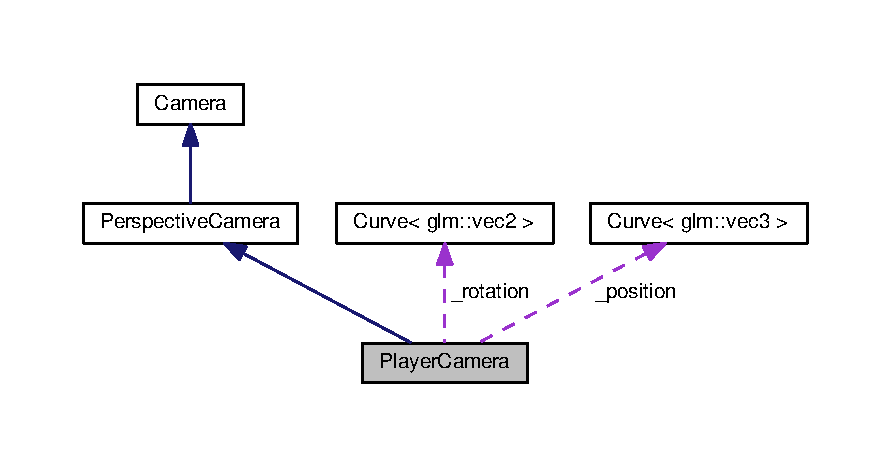
\includegraphics[width=350pt]{class_player_camera__coll__graph}
\end{center}
\end{figure}
\subsection*{Public Member Functions}
\begin{DoxyCompactItemize}
\item 
\hypertarget{class_player_camera_afcf71dc64aedd049567516a350f2d02e}{}{\bfseries Player\+Camera} (G\+L\+F\+Wwindow $\ast$window, float aspect)\label{class_player_camera_afcf71dc64aedd049567516a350f2d02e}

\item 
\hypertarget{class_player_camera_a525a7ad82ddb2fc7a5811064f70c128f}{}void {\bfseries add\+Collider} (\hyperlink{class_collider}{Collider} $\ast$collider)\label{class_player_camera_a525a7ad82ddb2fc7a5811064f70c128f}

\item 
\hypertarget{class_player_camera_ab6b201da5ff54012dc1a83281ce0cb47}{}void {\bfseries remove\+Collider} (\hyperlink{class_collider}{Collider} $\ast$collider)\label{class_player_camera_ab6b201da5ff54012dc1a83281ce0cb47}

\item 
\hypertarget{class_player_camera_a4b8f46b1603602471711ee4859c08ce2}{}virtual void {\bfseries step} (double dt)\label{class_player_camera_a4b8f46b1603602471711ee4859c08ce2}

\item 
\hypertarget{class_player_camera_a07e07be4973f01f696ab9cd2cc1d7fdc}{}void {\bfseries jump} ()\label{class_player_camera_a07e07be4973f01f696ab9cd2cc1d7fdc}

\end{DoxyCompactItemize}
\subsection*{Protected Member Functions}
\begin{DoxyCompactItemize}
\item 
\hypertarget{class_player_camera_abcda08bdd8dd2764e65539bdfae09131}{}void {\bfseries poll\+Input} ()\label{class_player_camera_abcda08bdd8dd2764e65539bdfae09131}

\end{DoxyCompactItemize}
\subsection*{Protected Attributes}
\begin{DoxyCompactItemize}
\item 
\hypertarget{class_player_camera_a42928613b1630cb4ae4d0607ac97b245}{}bool {\bfseries \+\_\+can\+Jump}\label{class_player_camera_a42928613b1630cb4ae4d0607ac97b245}

\item 
\hypertarget{class_player_camera_a883b822fa2ad7dfbc12551db76fbee9e}{}std\+::vector$<$ \hyperlink{class_collider}{Collider} $\ast$ $>$ {\bfseries \+\_\+colliders}\label{class_player_camera_a883b822fa2ad7dfbc12551db76fbee9e}

\item 
\hypertarget{class_player_camera_a3c8a4894c9863274e696973c2e303e78}{}G\+L\+F\+Wwindow $\ast$ {\bfseries \+\_\+window}\label{class_player_camera_a3c8a4894c9863274e696973c2e303e78}

\item 
\hypertarget{class_player_camera_a1d23e13334832fb7ad78fff02e987feb}{}\hyperlink{class_curve}{Curve}$<$ glm\+::vec3 $>$ {\bfseries \+\_\+position}\label{class_player_camera_a1d23e13334832fb7ad78fff02e987feb}

\item 
\hypertarget{class_player_camera_a43bfc21e3f1d0f3f95f509f5a0f4aed4}{}\hyperlink{class_curve}{Curve}$<$ glm\+::vec2 $>$ {\bfseries \+\_\+rotation}\label{class_player_camera_a43bfc21e3f1d0f3f95f509f5a0f4aed4}

\end{DoxyCompactItemize}
\subsection*{Additional Inherited Members}


The documentation for this class was generated from the following files\+:\begin{DoxyCompactItemize}
\item 
src/camera.\+h\item 
src/camera.\+cpp\end{DoxyCompactItemize}

\hypertarget{class_point_light}{}\section{Point\+Light Class Reference}
\label{class_point_light}\index{Point\+Light@{Point\+Light}}
\subsection*{Public Attributes}
\begin{DoxyCompactItemize}
\item 
\hypertarget{class_point_light_a6dc6e70f9a91e8a6bbecf08707143cad}{}glm\+::vec3 {\bfseries position}\label{class_point_light_a6dc6e70f9a91e8a6bbecf08707143cad}

\item 
\hypertarget{class_point_light_a3ea5c72fc0aa24e9c7434d33b45c5fdb}{}glm\+::vec3 {\bfseries diffuse}\label{class_point_light_a3ea5c72fc0aa24e9c7434d33b45c5fdb}

\item 
\hypertarget{class_point_light_a5154d2f188525f9365ee9f988b1ec353}{}glm\+::vec3 {\bfseries specular}\label{class_point_light_a5154d2f188525f9365ee9f988b1ec353}

\item 
\hypertarget{class_point_light_a8ca1748db53411217b9462120098b7a1}{}glm\+::vec3 {\bfseries attenuation}\label{class_point_light_a8ca1748db53411217b9462120098b7a1}

\end{DoxyCompactItemize}


The documentation for this class was generated from the following file\+:\begin{DoxyCompactItemize}
\item 
src/lighting.\+h\end{DoxyCompactItemize}

\hypertarget{class_post_effect}{}\section{Post\+Effect Class Reference}
\label{class_post_effect}\index{Post\+Effect@{Post\+Effect}}


Inheritance diagram for Post\+Effect\+:\nopagebreak
\begin{figure}[H]
\begin{center}
\leavevmode
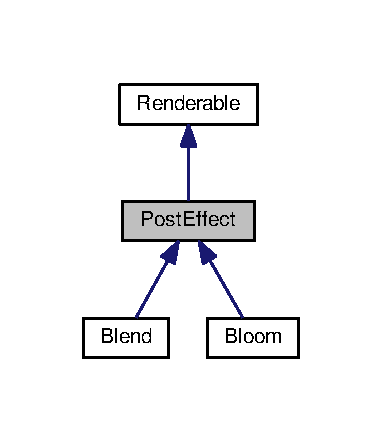
\includegraphics[width=184pt]{class_post_effect__inherit__graph}
\end{center}
\end{figure}


Collaboration diagram for Post\+Effect\+:\nopagebreak
\begin{figure}[H]
\begin{center}
\leavevmode
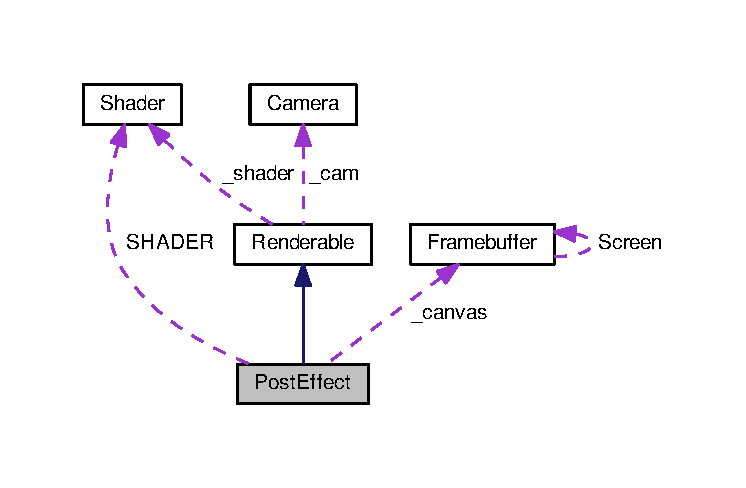
\includegraphics[width=350pt]{class_post_effect__coll__graph}
\end{center}
\end{figure}
\subsection*{Public Types}
\begin{DoxyCompactItemize}
\item 
\hypertarget{class_post_effect_aaccca6b80298db481b888abe761b0484}{}enum {\bfseries Type} \{ \\*
{\bfseries N\+O\+N\+E}, 
{\bfseries P\+I\+X\+E\+L\+A\+T\+E}, 
{\bfseries G\+A\+U\+S\+S\+\_\+\+V}, 
{\bfseries G\+A\+U\+S\+S\+\_\+\+H}, 
\\*
{\bfseries B\+L\+O\+O\+M\+\_\+\+F\+I\+L\+T\+E\+R}, 
{\bfseries B\+L\+E\+N\+D}
 \}\label{class_post_effect_aaccca6b80298db481b888abe761b0484}

\end{DoxyCompactItemize}
\subsection*{Public Member Functions}
\begin{DoxyCompactItemize}
\item 
\hypertarget{class_post_effect_a9e0e5cc2f6c226befa474e9275ed65da}{}{\bfseries Post\+Effect} (Type type, \hyperlink{class_framebuffer}{Framebuffer} $\ast$canvas)\label{class_post_effect_a9e0e5cc2f6c226befa474e9275ed65da}

\item 
\hypertarget{class_post_effect_a7274d736bac1655cc0e38e5fdf0dcf20}{}virtual void {\bfseries render} ()\label{class_post_effect_a7274d736bac1655cc0e38e5fdf0dcf20}

\item 
\hypertarget{class_post_effect_a79e9feb3a6a7f9a6d7d386edf80045a9}{}void {\bfseries set\+Type} (Type type)\label{class_post_effect_a79e9feb3a6a7f9a6d7d386edf80045a9}

\item 
\hypertarget{class_post_effect_a9a95d6d2be5272def9d246d1be702a72}{}void {\bfseries set\+Canvas} (\hyperlink{class_framebuffer}{Framebuffer} $\ast$canvas)\label{class_post_effect_a9a95d6d2be5272def9d246d1be702a72}

\end{DoxyCompactItemize}
\subsection*{Static Public Attributes}
\begin{DoxyCompactItemize}
\item 
\hypertarget{class_post_effect_ac3d05fdd220022ed1fe991488e246f4f}{}static \hyperlink{class_shader}{Shader} $\ast$ {\bfseries S\+H\+A\+D\+E\+R} = 0\label{class_post_effect_ac3d05fdd220022ed1fe991488e246f4f}

\end{DoxyCompactItemize}
\subsection*{Protected Attributes}
\begin{DoxyCompactItemize}
\item 
\hypertarget{class_post_effect_a674a1249e292efc6493dd612e7a96fd8}{}Type {\bfseries \+\_\+type}\label{class_post_effect_a674a1249e292efc6493dd612e7a96fd8}

\item 
\hypertarget{class_post_effect_a47c4b370fe5cdb4770555261476c0fcb}{}\hyperlink{class_framebuffer}{Framebuffer} $\ast$ {\bfseries \+\_\+canvas}\label{class_post_effect_a47c4b370fe5cdb4770555261476c0fcb}

\item 
\hypertarget{class_post_effect_a9df8cf2b75b102fc552c257d30cb739e}{}G\+Luint {\bfseries \+\_\+vbo}\label{class_post_effect_a9df8cf2b75b102fc552c257d30cb739e}

\end{DoxyCompactItemize}


The documentation for this class was generated from the following files\+:\begin{DoxyCompactItemize}
\item 
src/posteffect.\+h\item 
src/posteffect.\+cpp\end{DoxyCompactItemize}

\hypertarget{class_renderable}{}\section{Renderable Class Reference}
\label{class_renderable}\index{Renderable@{Renderable}}


Inheritance diagram for Renderable\+:\nopagebreak
\begin{figure}[H]
\begin{center}
\leavevmode
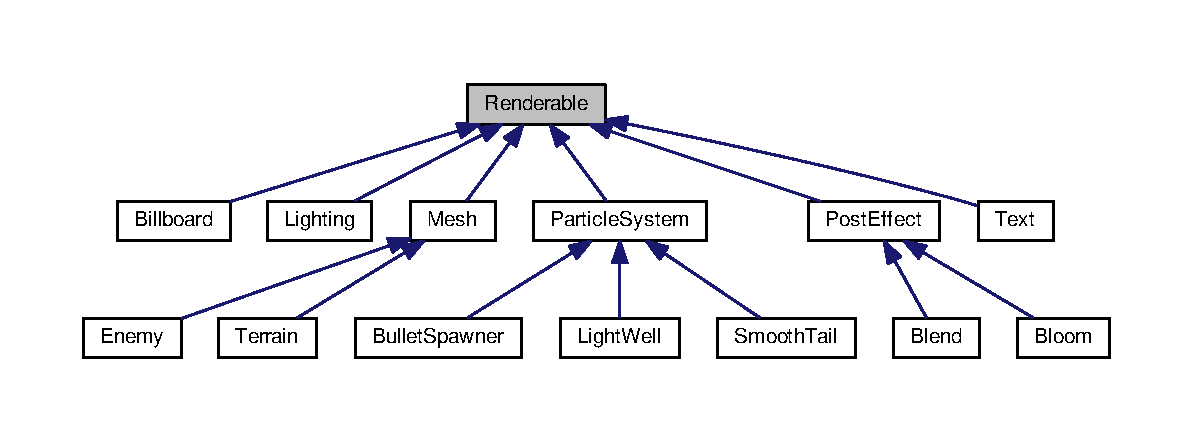
\includegraphics[width=350pt]{class_renderable__inherit__graph}
\end{center}
\end{figure}


Collaboration diagram for Renderable\+:\nopagebreak
\begin{figure}[H]
\begin{center}
\leavevmode
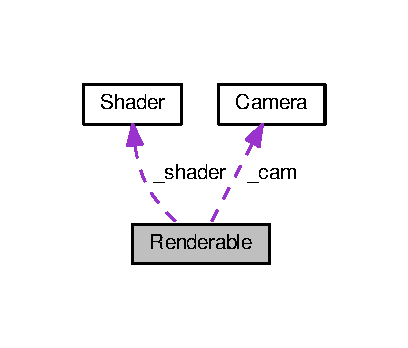
\includegraphics[width=196pt]{class_renderable__coll__graph}
\end{center}
\end{figure}
\subsection*{Public Member Functions}
\begin{DoxyCompactItemize}
\item 
\hypertarget{class_renderable_a337616d887f84c30a13fa9b37dea736a}{}{\bfseries Renderable} (\hyperlink{class_camera}{Camera} $\ast$cam, \hyperlink{class_shader}{Shader} $\ast$shader, G\+Luint vao, G\+Luint mode, size\+\_\+t elements, bool indexed)\label{class_renderable_a337616d887f84c30a13fa9b37dea736a}

\item 
\hypertarget{class_renderable_a1b807ee05938adc9b81ba9b15cfd66d8}{}void {\bfseries gen\+V\+A\+O} (std\+::vector$<$ \hyperlink{class_attribute}{Attribute} $>$ attributes, G\+Luint index\+Buffer)\label{class_renderable_a1b807ee05938adc9b81ba9b15cfd66d8}

\item 
\hypertarget{class_renderable_a1dce45c4703b60fd30acf824c77df9b6}{}virtual void {\bfseries render} ()\label{class_renderable_a1dce45c4703b60fd30acf824c77df9b6}

\end{DoxyCompactItemize}
\subsection*{Protected Attributes}
\begin{DoxyCompactItemize}
\item 
\hypertarget{class_renderable_aa0d63de6e1ff200bedf42fe598770ecc}{}\hyperlink{class_shader}{Shader} $\ast$ {\bfseries \+\_\+shader}\label{class_renderable_aa0d63de6e1ff200bedf42fe598770ecc}

\item 
\hypertarget{class_renderable_abd0605b721dfd91570553e59934d5c36}{}G\+Luint {\bfseries \+\_\+vao}\label{class_renderable_abd0605b721dfd91570553e59934d5c36}

\item 
\hypertarget{class_renderable_a8d09b0daa5ca8547d48e2bf464818461}{}G\+Lenum {\bfseries \+\_\+mode}\label{class_renderable_a8d09b0daa5ca8547d48e2bf464818461}

\item 
\hypertarget{class_renderable_a82ef267d43ff2396e4676ababbaacf74}{}size\+\_\+t {\bfseries \+\_\+elements}\label{class_renderable_a82ef267d43ff2396e4676ababbaacf74}

\item 
\hypertarget{class_renderable_ac35a8d537a915b392195b2d35f3fbf23}{}bool {\bfseries \+\_\+indexed}\label{class_renderable_ac35a8d537a915b392195b2d35f3fbf23}

\item 
\hypertarget{class_renderable_a6fee6e5a1d0181d37ce1eb5fb47278ee}{}\hyperlink{class_camera}{Camera} $\ast$ {\bfseries \+\_\+cam}\label{class_renderable_a6fee6e5a1d0181d37ce1eb5fb47278ee}

\item 
\hypertarget{class_renderable_a93095af76e9ef9da9c07bb8e91aa85da}{}G\+Lenum {\bfseries \+\_\+index\+Type} = G\+L\+\_\+\+U\+N\+S\+I\+G\+N\+E\+D\+\_\+\+S\+H\+O\+R\+T\label{class_renderable_a93095af76e9ef9da9c07bb8e91aa85da}

\item 
\hypertarget{class_renderable_a05b860b3426a5f6bc27c734d23bb26bd}{}G\+Lint {\bfseries \+\_\+start\+Index} = 0\label{class_renderable_a05b860b3426a5f6bc27c734d23bb26bd}

\end{DoxyCompactItemize}


The documentation for this class was generated from the following files\+:\begin{DoxyCompactItemize}
\item 
src/renderable.\+h\item 
src/renderable.\+cpp\end{DoxyCompactItemize}

\hypertarget{class_shader}{}\section{Shader Class Reference}
\label{class_shader}\index{Shader@{Shader}}
\subsection*{Public Types}
\begin{DoxyCompactItemize}
\item 
\hypertarget{class_shader_a2ac80773f1fe928469ce4ad5f9a05035}{}enum {\bfseries Load\+Flag} \{ {\bfseries L\+O\+A\+D\+\_\+\+B\+A\+S\+I\+C} = 0, 
{\bfseries L\+O\+A\+D\+\_\+\+G\+E\+O\+M} = 0x01, 
{\bfseries L\+O\+A\+D\+\_\+\+T\+E\+S\+S} = 0x02, 
{\bfseries L\+O\+A\+D\+\_\+\+F\+U\+L\+L} = 0x03
 \}\label{class_shader_a2ac80773f1fe928469ce4ad5f9a05035}

\end{DoxyCompactItemize}
\subsection*{Public Member Functions}
\begin{DoxyCompactItemize}
\item 
\hyperlink{class_shader_a4448038b6c1f3aa797685728618c761e}{Shader} (const std\+::string \&shader\+Dir, Load\+Flag load\+Flags)
\item 
G\+Lint \hyperlink{class_shader_a2708a72dd82b3123cb77f1f1dfbbce09}{get\+Uniform\+Location} (const std\+::string \&name)
\item 
bool \hyperlink{class_shader_a71a0f88dafffbb3c3f0829e7a8c77abc}{set\+Uniform} (const std\+::string \&name, G\+Lint val)
\item 
\hypertarget{class_shader_a92000cd568b0afffce9d3b71e3953ce7}{}bool {\bfseries set\+Uniform} (const std\+::string \&name, G\+Lfloat val)\label{class_shader_a92000cd568b0afffce9d3b71e3953ce7}

\item 
\hypertarget{class_shader_a05f2c0f13bad7ade5e89dc7349f0af26}{}bool {\bfseries set\+Uniform} (const std\+::string \&name, const glm\+::vec2 \&val)\label{class_shader_a05f2c0f13bad7ade5e89dc7349f0af26}

\item 
\hypertarget{class_shader_ae3f3704fec39edddd64945711df93eb6}{}bool {\bfseries set\+Uniform} (const std\+::string \&name, const glm\+::vec3 \&val)\label{class_shader_ae3f3704fec39edddd64945711df93eb6}

\item 
\hypertarget{class_shader_a14631fcf5837fadd0ab6646338d8f11d}{}bool {\bfseries set\+Uniform} (const std\+::string \&name, const glm\+::vec4 \&val)\label{class_shader_a14631fcf5837fadd0ab6646338d8f11d}

\item 
\hypertarget{class_shader_a6bb527eba6c723f351e9427ea404f92f}{}bool {\bfseries set\+Uniform} (const std\+::string \&name, const glm\+::mat4 \&val)\label{class_shader_a6bb527eba6c723f351e9427ea404f92f}

\item 
\hypertarget{class_shader_a5e7a1c2b5e9cb47ba8f3f546e4c21081}{}{\bfseries operator G\+Luint} ()\label{class_shader_a5e7a1c2b5e9cb47ba8f3f546e4c21081}

\item 
\hypertarget{class_shader_a3ef07768420e3b9459cbe8d781868c76}{}G\+Luint {\bfseries get\+I\+D} () const \label{class_shader_a3ef07768420e3b9459cbe8d781868c76}

\end{DoxyCompactItemize}


\subsection{Constructor \& Destructor Documentation}
\hypertarget{class_shader_a4448038b6c1f3aa797685728618c761e}{}\index{Shader@{Shader}!Shader@{Shader}}
\index{Shader@{Shader}!Shader@{Shader}}
\subsubsection[{Shader(const std\+::string \&shader\+Dir, Load\+Flag load\+Flags)}]{\setlength{\rightskip}{0pt plus 5cm}Shader\+::\+Shader (
\begin{DoxyParamCaption}
\item[{const std\+::string \&}]{shader\+Dir, }
\item[{Load\+Flag}]{load\+Flags}
\end{DoxyParamCaption}
)}\label{class_shader_a4448038b6c1f3aa797685728618c761e}
Load a \hyperlink{class_shader}{Shader} from directory with the necessary files. The following naming convention is assumed\+: vertex shader\+: vert.\+glsl fragment shader\+: frag.\+glsl geometry shader\+: geom.\+glsl tesseval shader\+: eval.\+glsl tesscontrol shader\+: cont.\+glsl

These flags are used to specify the shader type\+: L\+O\+A\+D\+\_\+\+B\+A\+S\+I\+C \+: load fragment + vertex shader (always the case) L\+O\+A\+D\+\_\+\+G\+E\+O\+M \+: load geometry shader L\+O\+A\+D\+\_\+\+T\+E\+S\+S \+: load tesselation shader L\+O\+A\+D\+\_\+\+F\+U\+L\+L = L\+O\+A\+D\+\_\+\+G\+E\+O\+M $\vert$ L\+O\+A\+D\+\_\+\+T\+E\+S\+S \+: load tesselation and geometry shader


\begin{DoxyParams}{Parameters}
{\em shader\+Dir} & directory where the shader files are located \\
\hline
{\em load\+Flags} & specifies what kind of shaders should be loaded \\
\hline
\end{DoxyParams}


\subsection{Member Function Documentation}
\hypertarget{class_shader_a2708a72dd82b3123cb77f1f1dfbbce09}{}\index{Shader@{Shader}!get\+Uniform\+Location@{get\+Uniform\+Location}}
\index{get\+Uniform\+Location@{get\+Uniform\+Location}!Shader@{Shader}}
\subsubsection[{get\+Uniform\+Location(const std\+::string \&name)}]{\setlength{\rightskip}{0pt plus 5cm}G\+Lint Shader\+::get\+Uniform\+Location (
\begin{DoxyParamCaption}
\item[{const std\+::string \&}]{name}
\end{DoxyParamCaption}
)}\label{class_shader_a2708a72dd82b3123cb77f1f1dfbbce09}
Wrapper around gl\+Get\+Uniform\+Location() which also caches locations 
\begin{DoxyParams}{Parameters}
{\em name} & Name of the uniform variable \\
\hline
\end{DoxyParams}
\begin{DoxyReturn}{Returns}
-\/1 if the uniform wasn\textquotesingle{}t found, else the opengl location I\+D 
\end{DoxyReturn}


Here is the caller graph for this function\+:
\nopagebreak
\begin{figure}[H]
\begin{center}
\leavevmode
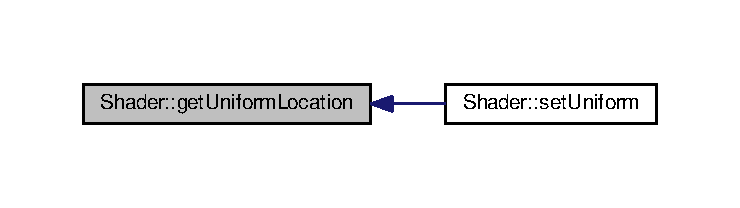
\includegraphics[width=350pt]{class_shader_a2708a72dd82b3123cb77f1f1dfbbce09_icgraph}
\end{center}
\end{figure}


\hypertarget{class_shader_a71a0f88dafffbb3c3f0829e7a8c77abc}{}\index{Shader@{Shader}!set\+Uniform@{set\+Uniform}}
\index{set\+Uniform@{set\+Uniform}!Shader@{Shader}}
\subsubsection[{set\+Uniform(const std\+::string \&name, G\+Lint val)}]{\setlength{\rightskip}{0pt plus 5cm}bool Shader\+::set\+Uniform (
\begin{DoxyParamCaption}
\item[{const std\+::string \&}]{name, }
\item[{G\+Lint}]{val}
\end{DoxyParamCaption}
)}\label{class_shader_a71a0f88dafffbb3c3f0829e7a8c77abc}
Bunch of Uniform setter functions which lookup the name with gl\+Get\+Uniform\+Location(). 
\begin{DoxyParams}{Parameters}
{\em name} & Name of the uniform variable \\
\hline
{\em val} & set the uniform to this value \\
\hline
\end{DoxyParams}
\begin{DoxyReturn}{Returns}
true on success, false on failure 
\end{DoxyReturn}


Here is the call graph for this function\+:\nopagebreak
\begin{figure}[H]
\begin{center}
\leavevmode
\includegraphics[width=350pt]{class_shader_a71a0f88dafffbb3c3f0829e7a8c77abc_cgraph}
\end{center}
\end{figure}




The documentation for this class was generated from the following files\+:\begin{DoxyCompactItemize}
\item 
src/shader.\+h\item 
src/shader.\+cpp\end{DoxyCompactItemize}

\hypertarget{class_smooth_tail}{}\section{Smooth\+Tail Class Reference}
\label{class_smooth_tail}\index{Smooth\+Tail@{Smooth\+Tail}}


Inheritance diagram for Smooth\+Tail\+:\nopagebreak
\begin{figure}[H]
\begin{center}
\leavevmode
\includegraphics[width=163pt]{class_smooth_tail__inherit__graph}
\end{center}
\end{figure}


Collaboration diagram for Smooth\+Tail\+:\nopagebreak
\begin{figure}[H]
\begin{center}
\leavevmode
\includegraphics[width=336pt]{class_smooth_tail__coll__graph}
\end{center}
\end{figure}
\subsection*{Public Member Functions}
\begin{DoxyCompactItemize}
\item 
\hypertarget{class_smooth_tail_a7935e55aa8afe863510c94dd6f98c559}{}{\bfseries Smooth\+Tail} (\hyperlink{class_perspective_camera}{Perspective\+Camera} $\ast$cam)\label{class_smooth_tail_a7935e55aa8afe863510c94dd6f98c559}

\item 
\hypertarget{class_smooth_tail_adcc5e45aec048cde4de7495e7a04f6ad}{}virtual void {\bfseries step} (double dt)\label{class_smooth_tail_adcc5e45aec048cde4de7495e7a04f6ad}

\end{DoxyCompactItemize}
\subsection*{Protected Attributes}
\begin{DoxyCompactItemize}
\item 
\hypertarget{class_smooth_tail_ab694a9acc9da93cd7c13e0bd453314b5}{}\hyperlink{class_curve}{Curve}$<$ glm\+::vec3 $>$ {\bfseries \+\_\+pos}\label{class_smooth_tail_ab694a9acc9da93cd7c13e0bd453314b5}

\end{DoxyCompactItemize}
\subsection*{Additional Inherited Members}


The documentation for this class was generated from the following files\+:\begin{DoxyCompactItemize}
\item 
src/particle.\+h\item 
src/particle.\+cpp\end{DoxyCompactItemize}

\hypertarget{class_sphere}{}\section{Sphere Class Reference}
\label{class_sphere}\index{Sphere@{Sphere}}


Inheritance diagram for Sphere\+:\nopagebreak
\begin{figure}[H]
\begin{center}
\leavevmode
\includegraphics[width=130pt]{class_sphere__inherit__graph}
\end{center}
\end{figure}


Collaboration diagram for Sphere\+:\nopagebreak
\begin{figure}[H]
\begin{center}
\leavevmode
\includegraphics[width=130pt]{class_sphere__coll__graph}
\end{center}
\end{figure}
\subsection*{Public Member Functions}
\begin{DoxyCompactItemize}
\item 
\hypertarget{class_sphere_a170af08dfd10bbafc0c3ec6fa693743e}{}{\bfseries Sphere} (glm\+::vec3 center, float radius)\label{class_sphere_a170af08dfd10bbafc0c3ec6fa693743e}

\item 
\hypertarget{class_sphere_a90f393174b2bb89987a35bf6144f93fe}{}virtual bool {\bfseries contains} (glm\+::vec3 point) const \label{class_sphere_a90f393174b2bb89987a35bf6144f93fe}

\item 
\hypertarget{class_sphere_aa451d786b6e46238c53bdc2a6799a10e}{}virtual glm\+::vec3 {\bfseries correct} (glm\+::vec3 point) const \label{class_sphere_aa451d786b6e46238c53bdc2a6799a10e}

\end{DoxyCompactItemize}
\subsection*{Protected Attributes}
\begin{DoxyCompactItemize}
\item 
\hypertarget{class_sphere_a8e01c6c14ad13dd80219430730ddac41}{}glm\+::vec3 {\bfseries \+\_\+center}\label{class_sphere_a8e01c6c14ad13dd80219430730ddac41}

\item 
\hypertarget{class_sphere_a73ecfaa359b78657c92cc04a5f2bb5fd}{}float {\bfseries \+\_\+radius}\label{class_sphere_a73ecfaa359b78657c92cc04a5f2bb5fd}

\end{DoxyCompactItemize}


The documentation for this class was generated from the following files\+:\begin{DoxyCompactItemize}
\item 
src/collider.\+h\item 
src/collider.\+cpp\end{DoxyCompactItemize}

\hypertarget{class_terrain}{}\section{Terrain Class Reference}
\label{class_terrain}\index{Terrain@{Terrain}}


Inheritance diagram for Terrain\+:\nopagebreak
\begin{figure}[H]
\begin{center}
\leavevmode
\includegraphics[width=202pt]{class_terrain__inherit__graph}
\end{center}
\end{figure}


Collaboration diagram for Terrain\+:\nopagebreak
\begin{figure}[H]
\begin{center}
\leavevmode
\includegraphics[width=316pt]{class_terrain__coll__graph}
\end{center}
\end{figure}
\subsection*{Public Member Functions}
\begin{DoxyCompactItemize}
\item 
\hypertarget{class_terrain_a985fd8481311a5d894620ff6261ca121}{}{\bfseries Terrain} (\hyperlink{class_camera}{Camera} $\ast$cam, \hyperlink{class_height_map}{Height\+Map} $\ast$heightmap, G\+Luint texture)\label{class_terrain_a985fd8481311a5d894620ff6261ca121}

\item 
\hypertarget{class_terrain_a56992faf594dadfdf2264c2f524ea12f}{}virtual void {\bfseries render} ()\label{class_terrain_a56992faf594dadfdf2264c2f524ea12f}

\item 
\hypertarget{class_terrain_aa907bd34d0c4abc859d95b4908f40b3c}{}virtual bool {\bfseries contains} (glm\+::vec3 point) const \label{class_terrain_aa907bd34d0c4abc859d95b4908f40b3c}

\item 
\hypertarget{class_terrain_a60d6629d3e3e525b5af4a041a5513804}{}virtual glm\+::vec3 {\bfseries correct} (glm\+::vec3 point) const \label{class_terrain_a60d6629d3e3e525b5af4a041a5513804}

\end{DoxyCompactItemize}
\subsection*{Static Public Attributes}
\begin{DoxyCompactItemize}
\item 
\hypertarget{class_terrain_a7160426f9fec0a57393977601b3e62de}{}static \hyperlink{class_shader}{Shader} $\ast$ {\bfseries S\+H\+A\+D\+E\+R} = 0\label{class_terrain_a7160426f9fec0a57393977601b3e62de}

\end{DoxyCompactItemize}
\subsection*{Protected Attributes}
\begin{DoxyCompactItemize}
\item 
\hypertarget{class_terrain_a09c59ff7e1157133d65a8bd44538da18}{}float {\bfseries \+\_\+width}\label{class_terrain_a09c59ff7e1157133d65a8bd44538da18}

\item 
\hypertarget{class_terrain_a4e90b826e3264d2587c7c30ebce7ad7e}{}float {\bfseries \+\_\+depth}\label{class_terrain_a4e90b826e3264d2587c7c30ebce7ad7e}

\item 
\hypertarget{class_terrain_aa126dea886f1c6d2f631c3547cfdf6ed}{}float {\bfseries \+\_\+max\+Height}\label{class_terrain_aa126dea886f1c6d2f631c3547cfdf6ed}

\item 
\hypertarget{class_terrain_a588e32d26d9219e693791ac05e14c458}{}\hyperlink{class_height_map}{Height\+Map} $\ast$ {\bfseries \+\_\+heightmap}\label{class_terrain_a588e32d26d9219e693791ac05e14c458}

\item 
\hypertarget{class_terrain_a41f2e7ff20e2e2f64bb4704db2dcc777}{}size\+\_\+t {\bfseries \+\_\+quad\+Count}\label{class_terrain_a41f2e7ff20e2e2f64bb4704db2dcc777}

\item 
\hypertarget{class_terrain_abb35500afa68d004491e95db62b7fcdf}{}G\+Luint {\bfseries \+\_\+buffers} \mbox{[}2\mbox{]}\label{class_terrain_abb35500afa68d004491e95db62b7fcdf}

\end{DoxyCompactItemize}


The documentation for this class was generated from the following files\+:\begin{DoxyCompactItemize}
\item 
src/terrain.\+h\item 
src/collider.\+cpp\item 
src/terrain.\+cpp\end{DoxyCompactItemize}

\hypertarget{class_text}{}\section{Text Class Reference}
\label{class_text}\index{Text@{Text}}


Inheritance diagram for Text\+:\nopagebreak
\begin{figure}[H]
\begin{center}
\leavevmode
\includegraphics[width=146pt]{class_text__inherit__graph}
\end{center}
\end{figure}


Collaboration diagram for Text\+:\nopagebreak
\begin{figure}[H]
\begin{center}
\leavevmode
\includegraphics[width=273pt]{class_text__coll__graph}
\end{center}
\end{figure}
\subsection*{Public Member Functions}
\begin{DoxyCompactItemize}
\item 
\hypertarget{class_text_ae77cabfcffef90b4a499f7c9f4f389ed}{}{\bfseries Text} (\hyperlink{class_font}{Font} $\ast$font, std\+::string text, glm\+::vec2 screen)\label{class_text_ae77cabfcffef90b4a499f7c9f4f389ed}

\item 
\hypertarget{class_text_a8a365f1337c52ee44e006bd59b82ff28}{}virtual void {\bfseries render} ()\label{class_text_a8a365f1337c52ee44e006bd59b82ff28}

\item 
\hypertarget{class_text_ab79897712890e561aadd14f38b3c64aa}{}virtual void {\bfseries on\+Resize} (int width, int height)\label{class_text_ab79897712890e561aadd14f38b3c64aa}

\item 
\hypertarget{class_text_ae479c13afc074e0b214a838bf27630aa}{}void {\bfseries set\+Position} (glm\+::vec2 pos)\label{class_text_ae479c13afc074e0b214a838bf27630aa}

\item 
\hypertarget{class_text_ae7d2d73938fedf4ea508b1eb827c72cd}{}glm\+::vec2 {\bfseries get\+Position} ()\label{class_text_ae7d2d73938fedf4ea508b1eb827c72cd}

\end{DoxyCompactItemize}
\subsection*{Static Public Attributes}
\begin{DoxyCompactItemize}
\item 
\hypertarget{class_text_a748a0c099aad9bec820278c28a3f4213}{}static \hyperlink{class_shader}{Shader} $\ast$ {\bfseries S\+H\+A\+D\+E\+R} = 0\label{class_text_a748a0c099aad9bec820278c28a3f4213}

\end{DoxyCompactItemize}
\subsection*{Protected Attributes}
\begin{DoxyCompactItemize}
\item 
\hypertarget{class_text_a8c902f985ee14e1ea4bfb5ff62f2d249}{}\hyperlink{class_font}{Font} $\ast$ {\bfseries \+\_\+font}\label{class_text_a8c902f985ee14e1ea4bfb5ff62f2d249}

\item 
\hypertarget{class_text_aa7182632b7555d834ccab02387ce8a22}{}G\+Luint {\bfseries \+\_\+buffers} \mbox{[}3\mbox{]}\label{class_text_aa7182632b7555d834ccab02387ce8a22}

\item 
\hypertarget{class_text_a8c4ad6de5b87e93c16bc50f6e65191e8}{}glm\+::vec2 {\bfseries \+\_\+screen}\label{class_text_a8c4ad6de5b87e93c16bc50f6e65191e8}

\item 
\hypertarget{class_text_adf2f5062284b46c3dcd66e81835d493e}{}glm\+::vec2 {\bfseries \+\_\+pos}\label{class_text_adf2f5062284b46c3dcd66e81835d493e}

\end{DoxyCompactItemize}


The documentation for this class was generated from the following files\+:\begin{DoxyCompactItemize}
\item 
src/text.\+h\item 
src/text.\+cpp\end{DoxyCompactItemize}

\hypertarget{class_texture}{}\section{Texture Class Reference}
\label{class_texture}\index{Texture@{Texture}}


Collaboration diagram for Texture\+:\nopagebreak
\begin{figure}[H]
\begin{center}
\leavevmode
\includegraphics[width=169pt]{class_texture__coll__graph}
\end{center}
\end{figure}
\subsection*{Public Member Functions}
\begin{DoxyCompactItemize}
\item 
\hyperlink{class_texture_a6c275e3f186675ff6ed73ccf970e552f}{Texture} ()
\item 
\hyperlink{class_texture_af0e04d16bacfbc9d1e52425efba4d898}{Texture} (G\+Luint id)
\item 
\hyperlink{class_texture_a09c4bcb7462f64c1d20fa69dba3cee8a}{$\sim$\+Texture} ()
\item 
void \hyperlink{class_texture_a49f3f1d6ec4370accdd9f007bb8934a5}{bind} () const 
\item 
void \hyperlink{class_texture_a0077a1cdcaf1c13e63f8f77f4894a84a}{set\+Internal\+Format} (G\+Lint internal\+Format)
\item 
void \hyperlink{class_texture_a7371169b17e32f6964af586ca6df2ff9}{set\+Format} (G\+Lenum format)
\item 
void \hyperlink{class_texture_a6819dd6a1070f0984d0c1f3c4ac47b22}{set\+Target} (G\+Lenum target)
\item 
void \hyperlink{class_texture_acd393734de22cd6e9f509f9ed41df8c0}{set\+Parameter} (G\+Lenum name, G\+Lint param) const 
\item 
void \hyperlink{class_texture_ab313b1279fda778b9575775f11392fcc}{set\+Parameter} (G\+Lenum name, G\+Lfloat param) const 
\item 
\hypertarget{class_texture_ac87726651e36811e1a46a0672d8a78a8}{}void {\bfseries load\+From\+File} (const std\+::string \&path)\label{class_texture_ac87726651e36811e1a46a0672d8a78a8}

\item 
void \hyperlink{class_texture_a7dbb3df1197eb229899158a128306d58}{load\+Data} (float $\ast$data) const 
\item 
void \hyperlink{class_texture_a11d626cb2c9fc19ed4946499832bce6c}{load\+Data} (unsigned short $\ast$data) const 
\item 
void \hyperlink{class_texture_a13edfe27037666e4fa7eeead51b29374}{load\+Data} (unsigned char $\ast$data) const 
\item 
void \hyperlink{class_texture_a61b781eed5eba214c0957df09b81fef1}{resize} (int w, int h)
\item 
G\+Luint \hyperlink{class_texture_a2b8ae08dd8da13a82e5fba4e9d691d1c}{get\+I\+D} () const 
\item 
\hypertarget{class_texture_a464c8e0de6328cd069de0c74c1bc8c60}{}{\bfseries operator G\+Luint} ()\label{class_texture_a464c8e0de6328cd069de0c74c1bc8c60}

\end{DoxyCompactItemize}
\subsection*{Static Public Member Functions}
\begin{DoxyCompactItemize}
\item 
static const \hyperlink{class_texture}{Texture} $\ast$ \hyperlink{class_texture_a9213840a2a31164baa96f98b292130b3}{get\+Active} ()
\end{DoxyCompactItemize}
\subsection*{Static Public Attributes}
\begin{DoxyCompactItemize}
\item 
\hypertarget{class_texture_ad3d72b2cbb6e539c5939349ecd259211}{}static \hyperlink{class_texture}{Texture} \hyperlink{class_texture_ad3d72b2cbb6e539c5939349ecd259211}{Null} = \hyperlink{class_texture}{Texture}( 0 )\label{class_texture_ad3d72b2cbb6e539c5939349ecd259211}

\begin{DoxyCompactList}\small\item\em \hyperlink{class_texture_a49f3f1d6ec4370accdd9f007bb8934a5}{bind()} to this texture to unbind any previous texture \end{DoxyCompactList}\end{DoxyCompactItemize}
\subsection*{Protected Attributes}
\begin{DoxyCompactItemize}
\item 
\hypertarget{class_texture_a41a325eee929d2aae4ecb203cae2cfcf}{}int {\bfseries \+\_\+width}\label{class_texture_a41a325eee929d2aae4ecb203cae2cfcf}

\item 
\hypertarget{class_texture_a1961677c206e2d4a8af399a33c349daf}{}int {\bfseries \+\_\+height}\label{class_texture_a1961677c206e2d4a8af399a33c349daf}

\item 
\hypertarget{class_texture_af6563b9b08f4bf2749639eb4434c9c35}{}G\+Luint \hyperlink{class_texture_af6563b9b08f4bf2749639eb4434c9c35}{\+\_\+id}\label{class_texture_af6563b9b08f4bf2749639eb4434c9c35}

\begin{DoxyCompactList}\small\item\em open\+G\+L I\+D \end{DoxyCompactList}\item 
\hypertarget{class_texture_ab4b0131aa6a35ff7a31dad24e9166135}{}G\+Lint \hyperlink{class_texture_ab4b0131aa6a35ff7a31dad24e9166135}{\+\_\+internal\+Format}\label{class_texture_ab4b0131aa6a35ff7a31dad24e9166135}

\begin{DoxyCompactList}\small\item\em G\+L\+\_\+\+R\+G\+B16\+F G\+L\+\_\+\+R32\+F etc. \end{DoxyCompactList}\item 
\hypertarget{class_texture_ac2029735134ea1a2de41a03e2e757217}{}G\+Lenum \hyperlink{class_texture_ac2029735134ea1a2de41a03e2e757217}{\+\_\+format}\label{class_texture_ac2029735134ea1a2de41a03e2e757217}

\begin{DoxyCompactList}\small\item\em G\+L\+\_\+\+R\+G\+B G\+L\+\_\+\+R\+G\+B\+A etc. \end{DoxyCompactList}\item 
\hypertarget{class_texture_a7240922837a1cfca87b1a4841f5c0b93}{}G\+Lenum \hyperlink{class_texture_a7240922837a1cfca87b1a4841f5c0b93}{\+\_\+target}\label{class_texture_a7240922837a1cfca87b1a4841f5c0b93}

\begin{DoxyCompactList}\small\item\em G\+L\+\_\+\+T\+E\+X\+T\+U\+R\+E\+\_\+2\+D etc. \end{DoxyCompactList}\end{DoxyCompactItemize}


\subsection{Constructor \& Destructor Documentation}
\hypertarget{class_texture_a6c275e3f186675ff6ed73ccf970e552f}{}\index{Texture@{Texture}!Texture@{Texture}}
\index{Texture@{Texture}!Texture@{Texture}}
\subsubsection[{Texture()}]{\setlength{\rightskip}{0pt plus 5cm}Texture\+::\+Texture (
\begin{DoxyParamCaption}
{}
\end{DoxyParamCaption}
)}\label{class_texture_a6c275e3f186675ff6ed73ccf970e552f}
Default Constructor 

Here is the call graph for this function\+:\nopagebreak
\begin{figure}[H]
\begin{center}
\leavevmode
\includegraphics[width=350pt]{class_texture_a6c275e3f186675ff6ed73ccf970e552f_cgraph}
\end{center}
\end{figure}


\hypertarget{class_texture_af0e04d16bacfbc9d1e52425efba4d898}{}\index{Texture@{Texture}!Texture@{Texture}}
\index{Texture@{Texture}!Texture@{Texture}}
\subsubsection[{Texture(\+G\+Luint id)}]{\setlength{\rightskip}{0pt plus 5cm}Texture\+::\+Texture (
\begin{DoxyParamCaption}
\item[{G\+Luint}]{id}
\end{DoxyParamCaption}
)}\label{class_texture_af0e04d16bacfbc9d1e52425efba4d898}
Doesn\textquotesingle{}t create I\+D but will delete \hyperlink{class_texture}{Texture} on destruction \hypertarget{class_texture_a09c4bcb7462f64c1d20fa69dba3cee8a}{}\index{Texture@{Texture}!````~Texture@{$\sim$\+Texture}}
\index{````~Texture@{$\sim$\+Texture}!Texture@{Texture}}
\subsubsection[{$\sim$\+Texture()}]{\setlength{\rightskip}{0pt plus 5cm}Texture\+::$\sim$\+Texture (
\begin{DoxyParamCaption}
{}
\end{DoxyParamCaption}
)}\label{class_texture_a09c4bcb7462f64c1d20fa69dba3cee8a}
Destructor 

\subsection{Member Function Documentation}
\hypertarget{class_texture_a49f3f1d6ec4370accdd9f007bb8934a5}{}\index{Texture@{Texture}!bind@{bind}}
\index{bind@{bind}!Texture@{Texture}}
\subsubsection[{bind() const }]{\setlength{\rightskip}{0pt plus 5cm}void Texture\+::bind (
\begin{DoxyParamCaption}
{}
\end{DoxyParamCaption}
) const}\label{class_texture_a49f3f1d6ec4370accdd9f007bb8934a5}
gl\+Bind\+Texture() wrapper which also sets the Active variable obtained by \hyperlink{class_texture_a9213840a2a31164baa96f98b292130b3}{get\+Active()} 

Here is the caller graph for this function\+:
\nopagebreak
\begin{figure}[H]
\begin{center}
\leavevmode
\includegraphics[width=350pt]{class_texture_a49f3f1d6ec4370accdd9f007bb8934a5_icgraph}
\end{center}
\end{figure}


\hypertarget{class_texture_a9213840a2a31164baa96f98b292130b3}{}\index{Texture@{Texture}!get\+Active@{get\+Active}}
\index{get\+Active@{get\+Active}!Texture@{Texture}}
\subsubsection[{get\+Active()}]{\setlength{\rightskip}{0pt plus 5cm}const {\bf Texture} $\ast$ Texture\+::get\+Active (
\begin{DoxyParamCaption}
{}
\end{DoxyParamCaption}
)\hspace{0.3cm}{\ttfamily [static]}}\label{class_texture_a9213840a2a31164baa96f98b292130b3}
Get the currently bound texture \begin{DoxyReturn}{Returns}
the texture bound by the last call of \hyperlink{class_texture_a49f3f1d6ec4370accdd9f007bb8934a5}{bind()} 
\end{DoxyReturn}
\hypertarget{class_texture_a2b8ae08dd8da13a82e5fba4e9d691d1c}{}\index{Texture@{Texture}!get\+I\+D@{get\+I\+D}}
\index{get\+I\+D@{get\+I\+D}!Texture@{Texture}}
\subsubsection[{get\+I\+D() const }]{\setlength{\rightskip}{0pt plus 5cm}G\+Luint Texture\+::get\+I\+D (
\begin{DoxyParamCaption}
{}
\end{DoxyParamCaption}
) const}\label{class_texture_a2b8ae08dd8da13a82e5fba4e9d691d1c}
get open\+G\+L texture I\+D \hypertarget{class_texture_a7dbb3df1197eb229899158a128306d58}{}\index{Texture@{Texture}!load\+Data@{load\+Data}}
\index{load\+Data@{load\+Data}!Texture@{Texture}}
\subsubsection[{load\+Data(float $\ast$data) const }]{\setlength{\rightskip}{0pt plus 5cm}void Texture\+::load\+Data (
\begin{DoxyParamCaption}
\item[{float $\ast$}]{data}
\end{DoxyParamCaption}
) const}\label{class_texture_a7dbb3df1197eb229899158a128306d58}
gl\+Tex\+Image2\+D() wrapper 

Here is the call graph for this function\+:\nopagebreak
\begin{figure}[H]
\begin{center}
\leavevmode
\includegraphics[width=285pt]{class_texture_a7dbb3df1197eb229899158a128306d58_cgraph}
\end{center}
\end{figure}


\hypertarget{class_texture_a11d626cb2c9fc19ed4946499832bce6c}{}\index{Texture@{Texture}!load\+Data@{load\+Data}}
\index{load\+Data@{load\+Data}!Texture@{Texture}}
\subsubsection[{load\+Data(unsigned short $\ast$data) const }]{\setlength{\rightskip}{0pt plus 5cm}void Texture\+::load\+Data (
\begin{DoxyParamCaption}
\item[{unsigned short $\ast$}]{data}
\end{DoxyParamCaption}
) const}\label{class_texture_a11d626cb2c9fc19ed4946499832bce6c}
gl\+Tex\+Image2\+D() wrapper 

Here is the call graph for this function\+:\nopagebreak
\begin{figure}[H]
\begin{center}
\leavevmode
\includegraphics[width=285pt]{class_texture_a11d626cb2c9fc19ed4946499832bce6c_cgraph}
\end{center}
\end{figure}


\hypertarget{class_texture_a13edfe27037666e4fa7eeead51b29374}{}\index{Texture@{Texture}!load\+Data@{load\+Data}}
\index{load\+Data@{load\+Data}!Texture@{Texture}}
\subsubsection[{load\+Data(unsigned char $\ast$data) const }]{\setlength{\rightskip}{0pt plus 5cm}void Texture\+::load\+Data (
\begin{DoxyParamCaption}
\item[{unsigned char $\ast$}]{data}
\end{DoxyParamCaption}
) const}\label{class_texture_a13edfe27037666e4fa7eeead51b29374}
gl\+Tex\+Image2\+D() wrapper 

Here is the call graph for this function\+:\nopagebreak
\begin{figure}[H]
\begin{center}
\leavevmode
\includegraphics[width=285pt]{class_texture_a13edfe27037666e4fa7eeead51b29374_cgraph}
\end{center}
\end{figure}


\hypertarget{class_texture_a61b781eed5eba214c0957df09b81fef1}{}\index{Texture@{Texture}!resize@{resize}}
\index{resize@{resize}!Texture@{Texture}}
\subsubsection[{resize(int w, int h)}]{\setlength{\rightskip}{0pt plus 5cm}void Texture\+::resize (
\begin{DoxyParamCaption}
\item[{int}]{w, }
\item[{int}]{h}
\end{DoxyParamCaption}
)}\label{class_texture_a61b781eed5eba214c0957df09b81fef1}
Set the size of the texture 
\begin{DoxyParams}{Parameters}
{\em w} & the new width \\
\hline
{\em h} & the new height \\
\hline
\end{DoxyParams}


Here is the call graph for this function\+:\nopagebreak
\begin{figure}[H]
\begin{center}
\leavevmode
\includegraphics[width=272pt]{class_texture_a61b781eed5eba214c0957df09b81fef1_cgraph}
\end{center}
\end{figure}




Here is the caller graph for this function\+:\nopagebreak
\begin{figure}[H]
\begin{center}
\leavevmode
\includegraphics[width=350pt]{class_texture_a61b781eed5eba214c0957df09b81fef1_icgraph}
\end{center}
\end{figure}


\hypertarget{class_texture_a7371169b17e32f6964af586ca6df2ff9}{}\index{Texture@{Texture}!set\+Format@{set\+Format}}
\index{set\+Format@{set\+Format}!Texture@{Texture}}
\subsubsection[{set\+Format(\+G\+Lenum format)}]{\setlength{\rightskip}{0pt plus 5cm}void Texture\+::set\+Format (
\begin{DoxyParamCaption}
\item[{G\+Lenum}]{format}
\end{DoxyParamCaption}
)}\label{class_texture_a7371169b17e32f6964af586ca6df2ff9}
Sets the format used by gl\+Tex\+Image2\+D() 
\begin{DoxyParams}{Parameters}
{\em format} & One of the following\+: G\+L\+\_\+\+R\+E\+D, G\+L\+\_\+\+R\+G, G\+L\+\_\+\+R\+G\+B, G\+L\+\_\+\+B\+G\+R, G\+L\+\_\+\+R\+G\+B\+A, G\+L\+\_\+\+B\+G\+R\+A, G\+L\+\_\+\+R\+E\+D\+\_\+\+I\+N\+T\+E\+G\+E\+R, G\+L\+\_\+\+R\+G\+\_\+\+I\+N\+T\+E\+G\+E\+R, G\+L\+\_\+\+R\+G\+B\+\_\+\+I\+N\+T\+E\+G\+E\+R, G\+L\+\_\+\+B\+G\+R\+\_\+\+I\+N\+T\+E\+G\+E\+R, G\+L\+\_\+\+R\+G\+B\+A\+\_\+\+I\+N\+T\+E\+G\+E\+R, G\+L\+\_\+\+B\+G\+R\+A\+\_\+\+I\+N\+T\+E\+G\+E\+R, G\+L\+\_\+\+S\+T\+E\+N\+C\+I\+L\+\_\+\+I\+N\+D\+E\+X, G\+L\+\_\+\+D\+E\+P\+T\+H\+\_\+\+C\+O\+M\+P\+O\+N\+E\+N\+T, G\+L\+\_\+\+D\+E\+P\+T\+H\+\_\+\+S\+T\+E\+N\+C\+I\+L \\
\hline
\end{DoxyParams}


Here is the call graph for this function\+:\nopagebreak
\begin{figure}[H]
\begin{center}
\leavevmode
\includegraphics[width=290pt]{class_texture_a7371169b17e32f6964af586ca6df2ff9_cgraph}
\end{center}
\end{figure}


\hypertarget{class_texture_a0077a1cdcaf1c13e63f8f77f4894a84a}{}\index{Texture@{Texture}!set\+Internal\+Format@{set\+Internal\+Format}}
\index{set\+Internal\+Format@{set\+Internal\+Format}!Texture@{Texture}}
\subsubsection[{set\+Internal\+Format(\+G\+Lint internal\+Format)}]{\setlength{\rightskip}{0pt plus 5cm}void Texture\+::set\+Internal\+Format (
\begin{DoxyParamCaption}
\item[{G\+Lint}]{internal\+Format}
\end{DoxyParamCaption}
)}\label{class_texture_a0077a1cdcaf1c13e63f8f77f4894a84a}
Sets the internal format used by gl\+Tex\+Image2\+D() 
\begin{DoxyParams}{Parameters}
{\em internal\+Format} & base internal format, sized internal format or compressed internal format \\
\hline
\end{DoxyParams}


Here is the call graph for this function\+:\nopagebreak
\begin{figure}[H]
\begin{center}
\leavevmode
\includegraphics[width=322pt]{class_texture_a0077a1cdcaf1c13e63f8f77f4894a84a_cgraph}
\end{center}
\end{figure}


\hypertarget{class_texture_acd393734de22cd6e9f509f9ed41df8c0}{}\index{Texture@{Texture}!set\+Parameter@{set\+Parameter}}
\index{set\+Parameter@{set\+Parameter}!Texture@{Texture}}
\subsubsection[{set\+Parameter(\+G\+Lenum name, G\+Lint param) const }]{\setlength{\rightskip}{0pt plus 5cm}void Texture\+::set\+Parameter (
\begin{DoxyParamCaption}
\item[{G\+Lenum}]{name, }
\item[{G\+Lint}]{param}
\end{DoxyParamCaption}
) const}\label{class_texture_acd393734de22cd6e9f509f9ed41df8c0}
gl\+Tex\+Parameteri() wrapper 

Here is the call graph for this function\+:\nopagebreak
\begin{figure}[H]
\begin{center}
\leavevmode
\includegraphics[width=304pt]{class_texture_acd393734de22cd6e9f509f9ed41df8c0_cgraph}
\end{center}
\end{figure}




Here is the caller graph for this function\+:\nopagebreak
\begin{figure}[H]
\begin{center}
\leavevmode
\includegraphics[width=319pt]{class_texture_acd393734de22cd6e9f509f9ed41df8c0_icgraph}
\end{center}
\end{figure}


\hypertarget{class_texture_ab313b1279fda778b9575775f11392fcc}{}\index{Texture@{Texture}!set\+Parameter@{set\+Parameter}}
\index{set\+Parameter@{set\+Parameter}!Texture@{Texture}}
\subsubsection[{set\+Parameter(\+G\+Lenum name, G\+Lfloat param) const }]{\setlength{\rightskip}{0pt plus 5cm}void Texture\+::set\+Parameter (
\begin{DoxyParamCaption}
\item[{G\+Lenum}]{name, }
\item[{G\+Lfloat}]{param}
\end{DoxyParamCaption}
) const}\label{class_texture_ab313b1279fda778b9575775f11392fcc}
gl\+Tex\+Parameterf() wrapper 

Here is the call graph for this function\+:\nopagebreak
\begin{figure}[H]
\begin{center}
\leavevmode
\includegraphics[width=304pt]{class_texture_ab313b1279fda778b9575775f11392fcc_cgraph}
\end{center}
\end{figure}


\hypertarget{class_texture_a6819dd6a1070f0984d0c1f3c4ac47b22}{}\index{Texture@{Texture}!set\+Target@{set\+Target}}
\index{set\+Target@{set\+Target}!Texture@{Texture}}
\subsubsection[{set\+Target(\+G\+Lenum target)}]{\setlength{\rightskip}{0pt plus 5cm}void Texture\+::set\+Target (
\begin{DoxyParamCaption}
\item[{G\+Lenum}]{target}
\end{DoxyParamCaption}
)}\label{class_texture_a6819dd6a1070f0984d0c1f3c4ac47b22}
Sets the texture target, G\+L\+\_\+\+T\+E\+X\+T\+U\+R\+E\+\_\+2\+D is the default value 

Here is the call graph for this function\+:\nopagebreak
\begin{figure}[H]
\begin{center}
\leavevmode
\includegraphics[width=287pt]{class_texture_a6819dd6a1070f0984d0c1f3c4ac47b22_cgraph}
\end{center}
\end{figure}




The documentation for this class was generated from the following files\+:\begin{DoxyCompactItemize}
\item 
src/texture.\+h\item 
src/texture.\+cpp\end{DoxyCompactItemize}

\hypertarget{class_world}{}\section{World Class Reference}
\label{class_world}\index{World@{World}}


Collaboration diagram for World\+:\nopagebreak
\begin{figure}[H]
\begin{center}
\leavevmode
\includegraphics[width=350pt]{class_world__coll__graph}
\end{center}
\end{figure}
\subsection*{Public Member Functions}
\begin{DoxyCompactItemize}
\item 
\hypertarget{class_world_abb6603de9dbfae29ea5d68e0aaa595eb}{}{\bfseries World} (G\+L\+F\+Wwindow $\ast$window, int width, int height)\label{class_world_abb6603de9dbfae29ea5d68e0aaa595eb}

\item 
\hypertarget{class_world_a04f0e47d71b690d9934fa697fa27ad9d}{}void {\bfseries step} (double dt)\label{class_world_a04f0e47d71b690d9934fa697fa27ad9d}

\item 
\hypertarget{class_world_a150eab10c21532162bb698d72aecec16}{}void {\bfseries render} ()\label{class_world_a150eab10c21532162bb698d72aecec16}

\item 
\hypertarget{class_world_a792c151ca90c5324db0c3322201ad4c1}{}void {\bfseries on\+Resize} (int width, int height)\label{class_world_a792c151ca90c5324db0c3322201ad4c1}

\item 
\hypertarget{class_world_a320b4008798e9e4c3ea2a9d77106ef40}{}void {\bfseries on\+Key\+Action} (int key, int scancode, int action, int mods)\label{class_world_a320b4008798e9e4c3ea2a9d77106ef40}

\item 
\hypertarget{class_world_a63c6c3ebb8258168b85922eb65b84bc6}{}void {\bfseries on\+Mouse\+Move} (double x, double y)\label{class_world_a63c6c3ebb8258168b85922eb65b84bc6}

\end{DoxyCompactItemize}
\subsection*{Public Attributes}
\begin{DoxyCompactItemize}
\item 
\hypertarget{class_world_ab38e8711736900af0ff7c04f35cd8c5f}{}G\+L\+F\+Wwindow $\ast$ {\bfseries \+\_\+window}\label{class_world_ab38e8711736900af0ff7c04f35cd8c5f}

\item 
\hypertarget{class_world_a87118a50c3c186f00e9f54dcbd002045}{}int {\bfseries \+\_\+width}\label{class_world_a87118a50c3c186f00e9f54dcbd002045}

\item 
\hypertarget{class_world_aa7d9399fe3c52051f5fbcbcfeba30da8}{}int {\bfseries \+\_\+height}\label{class_world_aa7d9399fe3c52051f5fbcbcfeba30da8}

\item 
\hypertarget{class_world_ae58681644481e8f663ddc40a116e5c1c}{}\hyperlink{class_framebuffer}{Framebuffer} $\ast$ {\bfseries \+\_\+g\+Buffer}\label{class_world_ae58681644481e8f663ddc40a116e5c1c}

\item 
\hypertarget{class_world_af2c6b833b1b56799cfe2cfe2cf034ce9}{}\hyperlink{class_framebuffer}{Framebuffer} $\ast$ {\bfseries \+\_\+canvas}\label{class_world_af2c6b833b1b56799cfe2cfe2cf034ce9}

\item 
\hypertarget{class_world_aa6e4a4cc368f66127bc512e96072f33d}{}\hyperlink{class_framebuffer}{Framebuffer} $\ast$ {\bfseries \+\_\+bloomed}\label{class_world_aa6e4a4cc368f66127bc512e96072f33d}

\item 
\hypertarget{class_world_a86814ef77ecf2c4a4e22e9c31b9ef2ec}{}\hyperlink{class_mesh_data}{Mesh\+Data} {\bfseries \+\_\+sphere\+Data}\label{class_world_a86814ef77ecf2c4a4e22e9c31b9ef2ec}

\item 
\hypertarget{class_world_a50a2d8f6fc58e22d0fb233c594a8e41e}{}G\+Luint {\bfseries \+\_\+ground\+Tex}\label{class_world_a50a2d8f6fc58e22d0fb233c594a8e41e}

\item 
\hypertarget{class_world_a762ed7d2b821a8758bcf66c2bd1df844}{}\hyperlink{class_font}{Font} {\bfseries \+\_\+font}\label{class_world_a762ed7d2b821a8758bcf66c2bd1df844}

\item 
\hypertarget{class_world_a376c9c2961800cef60f4c6a5697249d0}{}double {\bfseries \+\_\+time}\label{class_world_a376c9c2961800cef60f4c6a5697249d0}

\item 
\hypertarget{class_world_a41d7fe11feb33f45c28c6beec25cecf6}{}size\+\_\+t {\bfseries \+\_\+score}\label{class_world_a41d7fe11feb33f45c28c6beec25cecf6}

\item 
\hypertarget{class_world_aff20ebc091e78248b5da276320940fca}{}\hyperlink{class_player_camera}{Player\+Camera} {\bfseries \+\_\+cam}\label{class_world_aff20ebc091e78248b5da276320940fca}

\item 
\hypertarget{class_world_a22b8f41ae05bcd239bfdb7e598fbf89d}{}\hyperlink{class_lighting}{Lighting} {\bfseries \+\_\+lighting}\label{class_world_a22b8f41ae05bcd239bfdb7e598fbf89d}

\item 
\hypertarget{class_world_a83081a0365622f65795c43baa5c71a0b}{}\hyperlink{class_bullet_spawner}{Bullet\+Spawner} {\bfseries \+\_\+bullets}\label{class_world_a83081a0365622f65795c43baa5c71a0b}

\item 
\hypertarget{class_world_a7265fce4e1994d1bca454fa2be12e77c}{}\hyperlink{class_light_well}{Light\+Well} {\bfseries \+\_\+lightwell}\label{class_world_a7265fce4e1994d1bca454fa2be12e77c}

\item 
\hypertarget{class_world_a5589b931efb38240e8a3581376e5fb8b}{}\hyperlink{class_height_map}{Height\+Map} {\bfseries \+\_\+heightmap}\label{class_world_a5589b931efb38240e8a3581376e5fb8b}

\item 
\hypertarget{class_world_ae670e228a727dc5aedf65eb026689633}{}\hyperlink{class_terrain}{Terrain} $\ast$ {\bfseries \+\_\+terrain}\label{class_world_ae670e228a727dc5aedf65eb026689633}

\item 
\hypertarget{class_world_a75b7ba1e6a667e2b2d6d621a470c3a97}{}std\+::vector$<$ \hyperlink{class_enemy}{Enemy} $\ast$ $>$ {\bfseries \+\_\+enemies}\label{class_world_a75b7ba1e6a667e2b2d6d621a470c3a97}

\item 
\hypertarget{class_world_a05234bbcb9027332684d294249f9663a}{}double {\bfseries \+\_\+spawn\+Frequency}\label{class_world_a05234bbcb9027332684d294249f9663a}

\item 
\hypertarget{class_world_a652133a3af10cc8ce6cd1f1d9a2dbd30}{}double {\bfseries \+\_\+spawn\+Timer}\label{class_world_a652133a3af10cc8ce6cd1f1d9a2dbd30}

\item 
\hypertarget{class_world_a93a99a7308e67ea269cef6263d728559}{}double {\bfseries \+\_\+fps}\label{class_world_a93a99a7308e67ea269cef6263d728559}

\end{DoxyCompactItemize}


The documentation for this class was generated from the following files\+:\begin{DoxyCompactItemize}
\item 
src/world.\+h\item 
src/world.\+cpp\end{DoxyCompactItemize}

%--- End generated contents ---

% Index
\backmatter
\newpage
\phantomsection
\clearemptydoublepage
\addcontentsline{toc}{chapter}{Index}
\printindex

\end{document}
